\documentclass[12pt]{report}
\usepackage[utf8]{inputenc}
\usepackage[english]{babel}
\usepackage{microtype}
\usepackage{libertine}
\usepackage{amsmath,amsthm}
\usepackage[varg]{newtxmath}
\usepackage{setspace,graphicx,epstopdf}
\usepackage{marginnote,datetime,url,enumitem,subfigure,rotating}
\usepackage{multirow}
\usepackage{xfrac}
\usepackage[openlevel=3]{bookmark}
\usepackage[tikz]{bclogo}
\usepackage{enumitem}

\setcounter{tocdepth}{2}

\def\D{\mathrm{d}}

\setlength{\parindent}{0ex}
\setlength{\parskip}{1em}%Espacement des par

\setlist[itemize]{topsep=-2pt}

\newcommand{\smalltodo}[2][] {\todo[caption={#2}, size=\scriptsize,%
fancyline, #1]{\begin{spacing}{.5}#2\end{spacing}}}
\newcommand{\rhs}[2][]{\smalltodo[color=green!30,#1]{{\bf PS:} #2}}

\newtheorem{theorem}{Theorem}[chapter]
\newtheorem{definition}{Definition}[chapter]
\newtheorem{remark}{Remark}[chapter]
\newtheorem{proposition}{Proposition}[chapter]

\newcommand{\E}[1]{\operatorname{E}\left[#1\right]}
\newcommand{\Et}[1]{\operatorname{E}_t\left[#1\right]}
\newcommand{\V}[1]{\operatorname{Var}\left[#1\right]}
\newcommand{\cov}[1]{\operatorname{Cov}\left(#1\right)}
\newcommand{\covt}[1]{\operatorname{Cov}_t\left(#1\right)}
\newcommand{\avg}[2]{\frac{#1}{#2} \sum_{i=#1}^{#2}}
\def\D{\mathrm{d}}
\newcommand{\Prob}[1]{\operatorname{Pr}\left[#1\right]}
\newcommand{\Probhat}[1]{\hat{\operatorname{Pr}}\left[#1\right]}
\newcommand{\plim}{\operatorname{plim}}
\newcommand{\pconv}{\overset{\text{p}}{\to}}
\newcommand{\dconv}{\overset{\text{d}}{\to}}
\newcommand{\msconv}{\overset{\text{ms}}{\to}}
\def\D{\mathrm{d}}


\begin{document}

\date{}
\title{\textbf{\huge{ECON8822 - Cross-Section and Panel Econometrics}}\\ \textit{Notes from Stefan Hoderlein's lectures}}
\author{Paul Anthony Sarkis\\ Boston College} 
 
\maketitle

\tableofcontents

\chapter{Nonparametrics}

\section{Quick refresh}

An econometric model's goal is to study the (causal) relationship between a dependent variable of interest and regressors. Regressors can play two role in economic analysis as they control the regression or are of direct interest.

Assume a linear model such that: $$Y = \alpha + X\beta + U $$ where $Y$ is the dependent variable 

\section{Kernel Density Estimation}

Density estimation might be interesting in its own right, when you need to identify the particular distribution of a random variable. Nevertheless, it is mostly studied as a fundamental building block for more complicated semi-/nonparametric models. Following the example in the previous section, suppose we want to estimate how $Y$ is related to $X$ where $$ Y = m_Y(X) + U $$ Then we recovered that, using the assumption that $m_Y(\cdot)$ is twice differentiable and bounded in its second-order derivative, as well as the assumption that $\E{U\vert X} = 0$, we have: $$\E{Y\vert X = x} = m_Y(x) = \int_\chi y\cdot f_{Y\vert X}(y, x)\D x $$ Moreover, from probability theory (Bayes' theorem): $$ \int_\chi y\cdot f_{Y\vert X}(y, x)\D x = \int_\chi y\cdot \frac{f_{YX}(y, x)}{f_{Y}(x)} \D x$$ where you have two density functions to estimate.

\subsection{Introductory examples}

Let $X$ be a random variable that can take the value of $1$ with true probability $p^0$ or $0$ else. Think of how you would estimate the probability $p^0$.

One answer is to draw the random variable many times and get a series $\{ x_1, x_2, ...\}$ then estimating $\hat p$ as the number of times we actually observed $1$ divided by the number of draws. Formally, if we perform $n$ random draws, $$\hat p = \frac{\sum_{i=1}^{n} \mathbb{I}\{x_i = 1\} }{n} $$ where $\mathbb{I}\{\cdot\}$ is a function that takes a value of 1 if the condition inside is true, 0 if not. For example, if one million draws are made and 333 333 of them have turned out to be ones, then: $\hat p = \frac{ 333333 }{1000000}\approx 1/3 $.

Now, let's assume $X$ is actually a continuous variable that can take any real value on its support. Thinking about the previous example, how would you estimate the probability that the realization of $X$ falls in a given interval of length $h$ around a given $x$, or more formally, falls in $[x - h/2, x+ h/2]$. This value $h$ is called the bandwidth.

Again, we could use the same strategy and draw the random variable $n$ times, counting the times $x_i$ falls in the ball around $x$ and compare it with the total number of draws: $$ \Probhat{ X\in B_{h/2}(x) } = \frac{\sum_{i=1}^{n} \mathbb{I}\{ x_i \in B_{h/2}(x)\} }{n} = \frac{1}{n} \sum_{i=1}^{n} \mathbb{I}\{ x - h/2 \leq x_i \leq x + h/2 \} $$

Is this type of estimator unbiased? We can check by looking at: $$\E{\Probhat{ X\in B_{h/2}(x) }} = \E{\mathbb{I}\{ x - h/2 \leq X \leq x + h/2 \}} = \Prob{X\in B_{h/2}(x)} $$ which shows that it is indeed an unbiased estimator. 

\subsection{Density estimation}

We have just seen how to estimate probabilities without making assumptions on any structure; in this subsection, we will see how it relates to estimating a density function.

First, think of what the pdf of $X$, denoted $f_X(x)$, actually is. It is the probability that $X$ takes the exact value $x$. In a sense, this is close to what we just did, however, we're looking for $X$ to be a point rather than in a set. The probability of being in a set is given by the cdf $F_X(x)$. It turns out that as we reduce the size of the set more and more, the two concept become closer and closer. Formally, as $h$ tends to 0, the set around $B_{h/2}(x)$ will only contain $x$. Since $f_X(x)$ is the derivative of $F_X(x)$, we can write: $$f_X(x) = \lim_{h\to 0} \frac{F_X(x+h/2) - F_X(x-h/2)}{h} = \lim_{h\to 0} \frac{\Prob{X\in B_{h/2}(x)}}{h} $$ where you should recognize the last term from the previous subsection.

And in fact, you could estimate the pdf by using the estimator for the probability as seen above: $$ \hat f_X(x) = \frac{\Probhat{X\in B_{h/2}(x)}}{h} = \frac{1}{nh} \sum_{i=1}^{n} \mathbb{I}\{ x - h/2 \leq x_i \leq x + h/2 \} $$ for a given $h$ that is relatively small (more about this later). We now have our first own density estimator, let's look at it in more detail.

The basic idea behind the estimator is to count how many observations fall in the neighborhood $x$, relative to the total number of observations, and the size of the neighborhood. Here we use ``count'' since our indicator function is rather naïve and only does that: setting a weight of one for observations in the neighborhood, and 0 for observations out of the neighborhood. The weight assignment function is called a kernel (hence the name of kernel density estimator). In particular, the one used above is called a uniform kernel because it assigns a uniform weight to all observations within the neighborhood. In practice, this is a very bad kernel and it should rarely be used. The parameter $h$ that defines the size of the neighborhood is called the bandwidth.

\subsection{Properties of Kernel Density Estimators}

\begin{definition}[Standard Kernel]
A standard kernel $K: \mathbb{R}\to\mathbb{R}_+$ is a non-negative function such that:\begin{itemize}
\item $\int K(\psi)\D \psi = 1$: the cdf of the kernel goes to one.
\item $\int \psi K(\psi)\D \psi = 0$: the kernel is symmetric around 0.
\item $\int K^2(\psi)\D \psi = \kappa_2 < \infty $:
\item $\int \psi^2 K(\psi)\D \psi = \mu_2 < \infty $: 
\end{itemize}
\end{definition}
You should view these properties through the lens of what we actually use a kernel for. Since a kernel is essentially a ``weight-assigning'' function, it must make sense that it is symmetric (equally off observations in either direction should be equally bad), that it is non-negative (although it might be interesting to assign negative weights to observations we really don't want) and that it stops assigning weights after a certain distance.

Using this definition, we can then define a kernel density estimator.
\begin{definition}[Rosenblatt-Parzen Kernel density estimator]
A Kernel density estimator for a given pdf $f_X(x)$ is defined as: $$ \hat f_X(x) = \frac{1}{nh} \sum_{i=1}^{n} K\left(\frac{x_i - x}{h}\right) $$ where $K(\cdot):\mathbb{R}\to\mathbb{R}_+$ is a standard kernel.
\end{definition}
\newpage
Interesting examples of kernels include:\begin{itemize}
\item Uniform kernel: $K(\psi) = \mathbb{I}\{\vert\psi\vert\leq 1/2\}$
\item Gaussian kernel: $K(\psi) = \frac{1}{\sqrt{2}}\exp\{- 0.5 \cdot \psi^2\}$
\item Epanechnikov kernel: $K(\psi) = \mathbb{I}\{\vert\psi\vert\leq 1\}\cdot (1 - \psi^2)\cdot (3/4) $
\end{itemize}

As we did in the parametric econometrics classes, we now look for the kernel density estimator properties such as bias and variance.

\subsubsection{Bias of the KDE}

Assume a random sampling over iid data. Then, $$\E{\hat f_X(x)} = \frac{1}{nh}\E{\sum_{i=1}^{n} K\left(\frac{x_i - x}{h}\right)} = \frac{1}{nh} \cdot n \cdot \E{ K\left(\frac{X - x}{h}\right)} $$ $$ = \frac{1}{h} \int K\left(\frac{\xi - x}{h}\right)\cdot f_X(\xi) \D\xi  $$ Then, we perform a change of variables such that the term inside the kernel is $\psi$, meaning $\xi = \psi h + x$ and $\D \xi = h\cdot \D \psi $. Replacing it in the bias formula we get:$$\E{\hat f_X(x)} = \frac{1}{h} \int K\left(\psi\right)\cdot f_X(\psi h + x) \cdot h\cdot  \D \psi = \int K\left(\psi\right)\cdot f_X(\psi h + x) \D \psi$$
Further, let's use a second order  mean value expansion to recover $f_X(x)$: $$f_X(\psi h + x) = f_X(x) + \psi h f_X'(x) + \frac{(\psi h)^2}{2}	 f_X''(x_r) $$ where $x_r$ includes a remainder term such that: $x_r = x + \lambda\psi h$. This yields us: 

\begin{align*}
\E{\hat f_X(x)} & = \int K\left(\psi\right)\cdot \left[ f_X(x) + \psi h f_X'(x) + \frac{(\psi h)^2}{2}	 f_X''(x_r)\right] \D \psi  
\end{align*}
\begin{align*}
& = \int K\left(\psi\right)\cdot f_X(x) \D \psi  + \int K\left(\psi\right)\cdot \psi h f_X'(x) \D \psi + \int K\left(\psi\right)\cdot \frac{(\psi h)^2}{2}	 f_X''(x_r) \D \psi \\ & = f_X(x) \underbrace{\int K\left(\psi\right)\cdot \D \psi}_{=1}  + h f_X'(x)\underbrace{\int K\left(\psi\right)\cdot \psi \D \psi}_{=0} + \frac{h^2}{2}\int K\left(\psi\right)\cdot \psi^2	 f_X''(x_r) \D \psi
\end{align*}
The last term is quite problematic since it cannot be simplified out of the integral. However, we know that $f_X''(x)$ could be, so we can naively subtract it and we'll see later that the remainder is actually not very relevant. $$ \frac{h^2}{2}\int K\left(\psi\right)\cdot \psi^2	 f_X''(x_r) \D \psi = \frac{h^2}{2} \int K\left(\psi\right)\cdot \psi^2	 (f_X''(x_r) - f_X''(x)) \D \psi $$ $$ + \frac{h^2}{2} \int K\left(\psi\right)\cdot \psi^2 f_X''(x) \D \psi $$ $$ = R + \frac{h^2}{2}  f_X''(x) \mu_2 $$ where $R$ is bounded by $o(h^2)$. Finally, we can write the expectation of our kernel density estimator as: $$ \E{\hat f_X(x)} = f_X(x) + \underbrace{\frac{h^2}{2}  f_X''(x) \mu_2 + o(h^2)}_{\operatorname{Bias}\left[\hat f_X(x)\right]} $$ and the bias is given by the last two terms. From this equation, you can see that the bias is increasing with the bandwidth. This is intuitive since a greater bandwidth also implies more observations that are not related to $x$ (global information) relative to the observations actually close to $x$ (local information). Global information being more likely to introduce bias in the estimator, $h$ is positively correlated with bias. In the opposite direction, the bias seems to disappear as $h$ goes to 0. This means that the estimator is more efficient when the bandwidth is very small, then why not make the bandwidth as small as possible? One could show by similar equation work that the variance of the estimator is given by: $$
\V{\hat f_X(x)} = \frac{1}{nh}  f_X(x) \kappa_2 + o((nh)^{-1}) $$
which this time is actually increasing as $h$ tends to 0. Again, intuitively this makes sense as reducing the size of the bandwidth will eventually reduce the number of observations and thus increase the variance. This phenomenon is called the bias-variance trade-off.

\subsubsection{Bias-variance trade-off}

In order to have a sense of what the bias and variance look like over the whole distribution, we integrate them with respect to $x$: $$\int \left(\operatorname{Bias}\left[\hat f_X(x)\right]\right)^2 \D x = c_1 \cdot h^4 \quad \int \V{\hat f_X(x)} \D x = c_2 \cdot (nh)^{-1} $$ This allows us to design an optimal measure of the trade-off, analogous to the mean squared error in the parametric case, defined as the Mean Integrated Squared Error: $\operatorname{MISE}(h) \equiv c_1 \cdot h^4 + c_2 \cdot (nh)^{-1} $. Now suppose we want to find the best bandwidth to minimize MISE: $$\frac{\partial MISE}{\partial h} = 0 \Leftrightarrow 4\cdot c_1\cdot h^3 - c_2\cdot n^{-1} h^{-2} = 0 \Leftrightarrow h \sim n^{-1/5} $$ meaning that $h$ must be proportional to $n^{-1/5}$. Again, this makes a lot of sense since it implies that increasing the number of observations allows you to reduce the size of the bands: the more observations you have, the more likely it is that they will fall around $x$, and thus the less need you have to keep wide bands.

\subsubsection{Asymptotics}

The rate of convergence of the KDE is $\sqrt{nh}$ where $n$ is the number of observations and $h$ the bandwidth. For an optimal bandwidth, we had $h = n^{-1/5}$, yielding a convergence rate of $\sqrt{n\cdot n^{-1/5}} = \sqrt{n^{4/5}} = n^{2/5}$. Therefore, the nonparametric estimator has a slower rate of convergence than its parametric counterparts of OLS and ML estimators.

\subsection{Going beyond the univariate, first-order KDE}

As we've seen, the KDE method is very interesting in how it gets around the lack of structure, but it creates a new trade-off between bias and variance. In order to reduce further the bias, one might be interested in increasing the dimensions of the kernels, to allow for capturing more data points.

\subsubsection{Density derivatives}

If $f_X(x)$ is a differentiable function of $x$, one could also use the derivative of the kernel to estimate the object. In practice, to estimate a $r$-th order derivative, a $r$-th order kernel would set all moments up to the $r$-th one to 0, and the $r$-th one as a finite moment $\mu_r$. This technique displays the advantage of having convergence at a rate closer to $\sqrt{n}$. However, you would get potentially negative tails (meaning it would not be a proper density), and the estimator would be very efficient in small samples.

\subsubsection{Multivariate Density estimation}

Another way of achieving bias reduction would be to use multivariate density estimation, meaning $X$ would now be a random vector in $\mathbb{R}^k$ space. The kernel density estimator would then be a product of all univariate kernels. Obviously, this method adds additional variation in the function, but you would need way more observations to get an interesting result. To see that, recall the intuition behind the kernel function: it assigns weights to observations based on the mean distance of these observations to a point of interest, given a bandwidth. It turns out that increasing the dimension of the neighborhood (from a line, to a square, to hypercubes) will also increase the volume of the object, thus reducing the probability of observations being near the point of interest, and increasing the need for observations. This problem is called the curse of dimensionality.

\section{Kernel Regression Estimation}

In the previous section, we were interested in estimating the distribution of one variable $X$. However, in most economics applications, a more interesting element to estimate is the distribution of a variable $Y$, conditional on $X$. This is the mean regression model that we are going to study here.

Recall our definition of a kernel density estimator for a true distribution $f_X(x)$: $$ \hat f_X(x) = \frac{1}{nh} \sum_{i=1}^{n} K\left(\frac{x_i - x}{h}\right) $$ where $K$ is a standard kernel (refer to ...). Also recall the mean regression model of $$\E{Y\vert X = x} = m_Y(x) = \int y\cdot \frac{f_{XY}(x, y)}{f_X(x)}\D y $$ Our goal is to use kernel density estimators for both the distribution of $X$ and the joint distribution of $X$ and $Y$. Formally, we look for: $$ \hat m_Y(x) = \int y\cdot \frac{\hat f_{XY}(x, y)}{\hat f_X(x)}\D y $$ 

\subsection{Nadaraya-Watson Estimator}

Intuitively, we turn directly to our kernel density estimators. We already wrote the definition of our estimator in the univariate case of estimating $\hat f_X(x)$, but what is the KDE for the joint distribution of $X$ and $Y$? For that we use a multivariate KDE including a product kernel. In particular, we get: $$\hat f_{XY}(x, y) = \frac{1}{nh^2} \sum_{i=1}^{n} \left( K\left(\frac{x_i - x}{h}\right)\cdot K\left(\frac{y_i - y}{h}\right)\right) $$ The two KDE can be used in the mean regression estimator to get: \begin{align*}
\hat m_Y(x) = \int y\cdot \frac{\hat f_{XY}(x, y)}{\hat f_X(x)}\D y & = \int y\cdot \frac{(nh^2)^{-1} \sum_{i=1}^{n} \left( K\left(\frac{x_i - x}{h}\right)\cdot K\left(\frac{y_i - y}{h}\right)\right)}{(nh)^{-1} \sum_{i=1}^{n} K\left(\frac{x_i - x}{h}\right)} \D y \\
& = \frac{1}{h}\cdot \frac{\sum_{i=1}^{n} K\left(\frac{x_i - x}{h}\right)\cdot \int y K\left(\frac{y_i - y}{h}\right)\D y }{\sum_{i=1}^{n} K\left(\frac{x_i - x}{h}\right)}  
\end{align*} The only term that is not obvious here is the last term of the numerator. Let's look at it in detail.

Apply a change of variable so that $\psi$ is the term inside the kernel. We get $y = \psi h + y_i$ (recall that since the kernel is symmetric $K(y_i - y) = K(y - y_i)$). We also have $\D y = h\D \psi$. Then we can write: $$ \int y K\left(\frac{y_i - y}{h}\right)\D y = \int (\psi h + y_i) K\left(\psi\right)h\D \psi $$ and separating we have: $$ h^2 \int \psi  K\left(\psi\right)\D \psi + h y_i \int K\left(\psi\right)\D \psi = h\cdot y_i $$ from the properties of the kernel. Finally, plugging this expression back into the mean regression estimator we get: $$ \hat m_Y(x) = \frac{\sum_{i=1}^{n} K\left(\frac{x_i - x}{h}\right)\cdot y_i }{\sum_{i=1}^{n} K\left(\frac{x_i - x}{h}\right)} $$

\begin{definition}[Nadaraya-Watson estimator]
For a given model of two variables $Y$ and $X$ such that $Y = m_Y(X) + U $, the Nadaraya-Watson estimator for the function $m_Y(x)$ is defined as: $$ \hat m_Y(x) = \frac{\sum_{i=1}^{n} K\left(\frac{x_i - x}{h}\right)\cdot y_i }{\sum_{i=1}^{n} K\left(\frac{x_i - x}{h}\right)} $$ where $K(\cdot):\mathbb{R}\to\mathbb{R}$ is a standard kernel.
\end{definition}

Note that a kernel regression estimator is only a valid estimator for $m(\cdot)$ in a local neighborhood of size $h$.

\subsubsection{Nadaraya-Watson and OLS}

Consider a model of $Y$ and $X$ such that $Y = \alpha + U$ or in matrix form: $$\begin{bmatrix}
Y_1 \\ \vdots \\ Y_N
\end{bmatrix} = \begin{bmatrix}
1 \\ \vdots \\ 1
\end{bmatrix}\cdot \alpha + \begin{bmatrix}
U_1 \\ \vdots \\ U_N
\end{bmatrix} $$ By OLS, the estimation of $\alpha$ is now straightforward: $$\hat\alpha = (\iota' \iota)^{-1} \iota' Y = \frac{\sum_i Y_i}{n} = \bar Y$$ where $\iota$ is a $n$-dimensional vector of 1. This means that the OLS estimation is equivalent to fitting a constant (the average of $Y$) globally on the model. Now, if you consider the NW estimator, you should see a type of relation between both. In fact, around the neighborhood of $x$, the two estimators are exactly the same. Hence, intuitively, you could see the NW estimator as fitting a constant locally for all $x$. To see that, reweight the the data by $K\left(\frac{x - X_i}{h}\right)^{1/2}$ so that observations in the neighborhood are 1, while others are 0 (in the case of the uniform kernel), the NW estimator is in fact the average of $Y$ for values of $Y$ inside of the neighborhood.

\subsection{Local OLS estimator}

We have seen that the intuition behind the NW estimator was about fitting a constant locally on the model. Naturally, one could think about extending this line of reasoning and fit more complex models inside the kernel. In particular, a well-studied extension is to fit a line, as a local linear model. This type of models is usually called local OLS models. They are represented by the following model: $$Y = m(x)\tilde\iota + h\cdot m'(x)\frac{X_i - x}{h} + U = \tilde X\beta (x) + U $$ Note that adding dimensions to the polynomial used to fit the model locally does not change the value of the $m(x)$ function, but rather adds information about higher-order derivatives of the $m(x)$ function at the point $x$. For example, estimating a simple line locally gives the value of the point at $x$ as well as the slope of $m$ at $x$.

\begin{definition}[Local OLS estimator]
For a given model of two variables $Y$ and $X$ such that $Y = m(x)\tilde\iota + h\cdot m'(x)\frac{X_i - x}{h} + U = \tilde X\beta (x) + U $, the local OLS estimator for the function $m_Y(x)$ is defined as:
$$\hat\beta(x) = (\tilde X'\tilde X)^{-1}\tilde X'\tilde Y $$
\end{definition}

\subsection{Bias and Variance}

The bias of the kernel regression estimation is given by: $$\E{\hat \beta_0\vert X} - \beta_0 = \E{\hat m(x)\vert X} - m(x) = \frac{h^2}{2} \cdot \mu_2 m_Y''(x) + o_p(h^2) $$ which is very similar to the formula derived for the bias of the kernel density estimator. If we also look at the variance, we get: $$\V{\hat \beta_0\vert X} = \V{\hat m(x)\vert X} = \frac{1}{nh}\cdot\kappa^2\frac{\sigma_U^2}{f_X(x)} + o_p((nh)^{-1}) $$ which is slightly different than the kernel density counterpart. In fact, in the regression case, $f_X(x)$ enters in the denominator, meaning that increasing $f(x)$ (the probability of finding observations at the point $x$) will decrease the variance while in the density estimation, increasing the number of observations increased the variance.

\subsection{General considerations}

\subsubsection{Asymptotic normality}

Under similar regularity conditions as the density estimator, the regression estimation will tend in distribution to a standard normal as the number of observations increase to $\infty$. The rate of convergence is also $\sqrt{nh}$ in this setting.

\subsubsection{Curse of dimensionality}

Again, in a similar way as the KDE, the kernel regression estimator faces the curse of dimensionality as the number of regressors $k$ increases. The rate of convergence is then $\sqrt{nh^k}$.

\subsubsection{Higher-order bias reduction}

Same as KDE.

\subsubsection{Order of local polynomial}

As it is discussed in the section, instead of fitting a constant or a line, one could go further and fit higher order polynomials in the data in order to get more information on the shape of the fitted line. It turns out that asymptotically, there is no cost to move to the next-odd order when estimating a given object of interest. For example, say you want to estimate $m(\cdot)$ up to its $p$-th derivative, then you could use a $p+1$ or $p+3$ order local polynomial estimation. You should remember that when it comes to local OLS, it is an odd world.

Moreover, estimating polynomials will actually achieve bias reduction in the same way that high order kernel do. This bias reduction comes without the cost of putting negative weight on some observations like the higher order kernels do. This is why it is generally thought that high order polynomial is more interesting than high order kernels.

\subsubsection{Selection of bandwidth}

There are two schools of thoughts when it comes to bandwidth selection in the case of kernel regression.

We have seen in the kernel density estimation section that we chose the bandwidth in order to minimize the mean integrated squared error. In the context of kernel regression, the MISE does not have an analytic expression, and we thus have to approximate it using the following expression: $$ AMISE = \int \frac{h^2}{2} \cdot \mu_2 m_Y''(x) + \frac{1}{nh}\cdot\kappa^2\frac{\sigma_U^2}{f_X(x)} \D x $$ and then minimize over $h$.

The second way to select the adequate bandwidth is to use cross-validations. Define the leave-one-out estimator $\hat m_{-j}$ as the the standard local OLS estimator, without the $j$-th observation. Now let the average prediction error (APE) be: $$APE = \frac{1}{n} \sum_j (Y_j - \hat m_{-j}(X_j))^2 $$ It turns out that choosing $h$ to minimize the APE is equivalent to minimizing the MISE.

\subsubsection{Choice of kernel}

Use Epanechnikov.

\subsection{Series/sieve regression}



\subsection{Testing}

In nonparametrics, hypothesis testing is separated from the regression estimation. It is also difficult to perform as generally, hypothesis testing is meant to look at interesting features on the whole dataset (the whole function), while nonparametrics focuses on local features of the data.

\subsubsection{Omission of variables test}

\subsection{Applications}

\subsubsection{Binary Dependent Variable}

Consider the case where $Y$, the dependent variable, only takes values of 1 or 0, such that: $$Y = \begin{cases}
1 & \text{ if } X\beta + U > 0 \\
0 & \text{ else.}
\end{cases}
$$ where $U$ is assumed to be independent of $X$, $U\perp X$.
As outlined in the beginning of this section, we look for an estimator for the expectation of $Y$ given $X = x$. Since $Y$ is now a discrete random variable, we can write: \begin{align*}
\E{Y\vert X = x} & = 1 \cdot \Prob{X\beta + U > 0\vert X = x} + 0 \cdot \Prob{X\beta + U \leq 0\vert X = x} \\
& = \Prob{X\beta + U > 0 \vert X = x} = \Prob{U > -x\beta}\\
& = 1 - G(-x\beta)
\end{align*}
This setting is problematic since it does not allow for ``point-identification'' of $\beta$. To see that, note that we have two objects to estimate here: $\theta = \{G(-X\beta), \beta\}$. However, we could also define $\tilde\beta = \beta/c$ and $\tilde G(z) = G(cz)$, which would yield that $\tilde G(X\tilde\beta) = G(X\beta)$. This means that observing the same data, one could estimate $\tilde G$ or $G$, leaving $\beta$ unidentified, or set identified (all vectors $\tilde\beta$). We say that $\beta$ is identified up to scale $c$.

In order to solve this issue, we can impose a restriction on the size of $\beta$ such that we can single out a parameter from all proportional parameters. We call this restriction a normalization. 

This normalization turns out not to affect the economic meaningfulness of the model. In fact, we have just seen that $G(\cdot)$ is perfectly identified, but identification of $\beta$, although an advantage, is not necessary. To see that, consider another object of interest in this model:
$$\triangledown_x \E{Y\vert X = x} = \beta \cdot  g(-x\beta) $$ where $g$ denotes the pdf of the distribution of $U$. Then, define the set of parameters we want to estimate as $\theta = \{G(X\beta), \beta g(X\beta)\}$. Now let $\tilde{\beta} = \beta/c$ and $\tilde{G}(x) = G(cx)$. From this we get that $G(-X\beta) = \tilde{G}(-X\tilde\beta)$ and $\beta g(-X\beta) = \tilde\beta\tilde g(-X\tilde\beta)$. Therefore, we can write that $\tilde\theta = \theta$, meaning that whatever the value of $c$ is, our set of objects of interest will not change.

\chapter{Treatment Effects}

\section{Intuition}

Suppose the data follows the model: $$ Y = \phi(D, A) $$ where $\phi(\cdot)$ is a very general function of the data, such that it is not differentiable; $D$ is the discrete (binary) variable indicating if yes (1) or no (0) the treatment was administered; and $A$ is a potentially infinite dimensional error.

We denote $Y_1$ and $Y_0$ as respectively the values of the outcome for each different treatment: $$Y_1 = \phi(1, A) ; \quad Y_0 = \phi(0, A) $$ Note that both variables are not (never) directly observed. The observations in the data are realized outcomes depending on the realization of the random variable $A$. Thus, the function $\phi$ that transforms the data can never be observed.

Ideally, we want to be able to recover the effect of the treatment, or how the outcome changes when $D=0$ increases to $D=1$, for a given $A = a$ (an individual). We call this the individual treatment effect: $$Y_1 - Y_0 = \phi(1, A) - \phi(0, A) $$ which varies for any $A$, across the population. However, knowing the effect for any individual might not be that useful in practical terms. In fact, when designing a policy or evaluating programs, you might be interested only in a subgroup of people, or the population as a whole, but rarely about each individual. This is why we might be more interested in the Average Treatment Effect (or ATE), defined as: $$ATE \equiv \E{Y_1 - Y_0} = \E{\phi(1, A) - \phi(0, A)} $$ the average of the individual treatment effect across all individuals. One could also be directly looking at the subgroup of interest, say the average treatment effect on the treated (ATT), i.e. $$ ATT \equiv \E{Y_1 - Y_0\vert D = 1} = \E{\phi(1, A) - \phi(0, A)\vert D=1} $$ Going further, one might be interested in identifying a subgroup on other characteristics $X$, using the average treatment effect conditional on $X$ (or CATE): $$CATE \equiv \E{Y_1 - Y_0\vert X = x} = \E{\phi(1, A) - \phi(0, A)\vert X=x} $$ Finally, in the same line of reasoning, one could separate subpopulations in terms of endogeneity of their response to the treatment, using estimators we'll study later like LATE, MTE, etc. All these estimators take the form: $$ \E{Y_1 - Y_0\vert \textit{Subpop.}} = \E{\phi(1, A) - \phi(0, A)\vert \textit{Subpop.}} $$

To go back to our first object of interest, an alternative interpretation of the average treatment effect can be found by rewriting the equation in terms of the binary variable: $$Y = \phi(D, A) = Y_0 + (Y_1 - Y_0)\cdot D = \alpha(A) + \beta(A)\cdot D $$ where $Y_0$ becomes a random intercept and $Y_1 - Y_0$ a random slope. Then, the ATE is the average random slope of the model: $ATE = \E{\beta(A)}$.

\section{Identification}

If $Y_1$ and $Y_0$ were known for the whole population under study, there would not be a whole field dedicated to compute the ATE. In fact, averaging over a simple substraction would be quite easy. However, for any individual $i$, only one of the outcomes can be observed at the same time. In fact, either an individual received the treatment ($Y_{1i}$ is observed) or he did not ($Y_{0i}$ is observed). Because of that fact, we will have to make some assumptions on the unobservables to make progress.

\subsection{Joint full independence}

In particular, the first assumption we ought to make is the so-called ``joint full independence'' of outcomes with respect to treatment. Formally, we write: $(Y_1, Y_0)\perp D$, meaning that jointly, $Y_1$ and $Y_0$ are fully independent from $D$. This also implies that $A\perp D$.

Intuitively, this assumption (denoted $A2$) means two things. First, that everything not observed by the econometrician ($A$) is independent of the treatment $D$, i.e. receiving the treatment or not does not change the unobserved variables that might affect the outcome of the treatment. Second, the unobserved variable $A$ has no effect on the treatment being delivered or not, i.e. the treatment is purely random, even on unobserved characteristics.

This assumption has an interesting implication on the regression of $Y$ on $D$. Consider the regression separated for each group of treatment. For the treated: \begin{align*}
\E{Y\vert D =1} & = \E{Y_0 + (Y_1 - Y_0)\cdot D\vert D = 1} \\ & = \E{Y_0 + (Y_1 - Y_0) \vert D = 1}  \\ & = \E{Y_1 \vert D = 1}  \\ & = \E{Y_1} \text{ by assumption of joint full independence.}
\end{align*} Similarly, for the non-treated, you get: $\E{Y\vert D = 0} = \E{Y_0} $. And thus, $$ ATE = \E{Y_1 - Y_0} = \E{Y_1} - \E{Y_0} = \E{Y\vert D =1} - \E{Y\vert D = 0} $$ In words, this assumption allows the econometrician to compute the ATE as the difference between the average effect across the treatment group ($\E{Y\vert D =1}$) and the average effect across the control group ($\E{Y\vert D =0}$). Remember that this can only be true if unobservables across the whole population are independent of the treatment.

Under the same assumption, we also get that $\E{Y\vert D =0} = \E{Y_0} = \E{Y_0\vert D =1}$ and thus $ ATE = ATT$.

\subsection{Unconfoundedness}

Although the previous assumption allows for some very interesting results, it requires a lot of effort to ensure. In fact, the assumption requires perfect randomization of the treatment assignment. This setting is called a perfect experiment, but it is not so common in research, as it is hard to randomize, and/or make sure that everyone follows the instructions. Nevertheless, we could study a more realistic setting where, conditional on some observables $X$, we would have independence. Assuming the following model:
$$ Y = \phi(D, X, A) = \alpha(A, X) + \beta(A, X)\cdot D $$ the unconfoundedness assumption ($A2'$) requires that $(Y_1, Y_0) \perp D\vert X $, implying that $A\perp D\vert X$, instead of the previous $A\perp D$. A weaker assumption ($A2''$) would be that only the expectations of $Y$ would be the same regardless of the treatment once conditioned on $X$ (more formally, $\E{Y_j\vert D, X} = \E{Y_j\vert X}$ for both $j = 0,1$).

Using this assumption and following the same reasoning as with joint full independence, we can come up with the Conditional Average Treatment Effect (CATE): \begin{align*} CATE(x) = \E{Y_1 - Y_0\vert X=x} & = \E{Y_1 \vert X=x} - \E{Y_0\vert X=x} \\ & = \E{Y \vert D=1, X=x} - \E{Y\vert D=0, X=x}
\end{align*}
and thus, the average treatment effect as: $$ATE = \int CATE(x) \D F(x) = \int \left(\E{Y \vert D=1, X=x} - \E{Y\vert D=0, X=x}\right)\D F(x) $$ which in words is the expectation of the CATE over $X$.

\subsubsection{Estimation}

This equation for the ATE should really ring a bell if you have followed the last chapter. In fact, both elements within the integral can be estimated with nonparametric (kernel) regression. However, this type of regression applied directly to the problem will throw you directly under the curse of dimensionality (having expectations conditional on both $D$ and $X$, the latter potentially being multidimensional as well).

A solution to this problem could be to implement a variable linking the treatment $D$ to the observables $X$. Define a propensity score $p(x) \equiv \Prob{D = 1\vert X = x}$. Along uncertainty in $X$, you get uncertainty in $p$, which can be summarized as a random variable $P$. Then, using the previous assumptions $A2'$, we get: $$ CATE(p) = \E{Y \vert D=1, P=p} - \E{Y\vert D=0, P=p} $$ where $P$ only has a single dimension.

In practice, this propensity score $p$ could be estimated nonparametrically or not. The issue with nonparametric estimation is that you are just displacing the dimensionality curse situation. Using a parametric structure such as the probit, logit or the kind would help in reducing the dimensionality issue.

Now, using the definition of the ATE, we have: $$ATE = \E{\E{Y \vert D=1, P=p} - \E{Y\vert D=0, P=p}}$$ $$\widehat{ATE} = \frac{1}{n} \sum_i \hat m_1(P_i) - \hat m_0(P_i) $$

\subsubsection{Practical issues}

Using last chapter, we know how to estimate $m(\cdot)$. Nevertheless, the setting derived just above is slightly different than before in the sense that the object of interest, $\widehat{ATE}$, is now an average over kernel regression estimators. Among other things, this changes how we interpret the optimal bandwidth. In fact, since we are now averaging, we could deal with smaller bandwidths without being too scared of the effect it would have on variance (averages reduce variances). Because a smaller $h$ is not that costly anymore, the cross-validation approach does not deliver the best bandwidth anymore, so we'll have to use different approaches. In particular, the field has come up with two interesting approaches: (1) the propensity score matching and (2) direct averages.

The propensity score matching is very intuitive and maps to a sort of nearest neighbor estimator. The idea is that for any individual $i$ in the control group (with propensity score $p_i$), you find the individual $i'$ in the treatment group such that $i'\in\arg\min_{j\in I_1} \vert p_i - p_j\vert$ where $I_1$ is the set of individual who received the treatment. In words, you "match" every individual in the control group with at least one individual in the treatment, based on the proximity of their proximity score. Then, for each pair you compute the difference between their CATE, and finally average over all pairs to get the ATE. The advantage in that estimator is that as $n$ increase, you will find more and more individuals in the matching pairs. However, one disadvantage is that even with an infinite number of individuals, the bias of this estimator will not vanish.

The second approach of direct averages uses a clever rewriting of the problem such that the ATE is defined as: $$ATE \equiv \E{\frac{(D - p(X))\cdot Y}{p(X)\cdot (1 - p(X)}} $$ which suggests the simple following sample counterpart: $$\widehat{ATE} \equiv \frac{1}{n}\sum_{i} \frac{(D_i - \hat p(X_i))\cdot Y_i}{\hat p(X_i)\cdot (1 - \hat p(X_i)} $$ where $\hat p(\cdot)$ can be any first-stage estimator of the propensity score (non-parametric, probit, etc.).

\subsection{Regression Discontinuity Design (RDD)}

The RDD is another setup used to analyze treatment effects conditional on covariates. The idea is quite simple and intuitive since it relies on an existing discontinuity in the treatment selection (who gets it and who do not) to study the effect of the treatment. In simpler words, if along a dataset the only discontinuity is whether a treatment was received or not (all other variables are continuous), then by studying the response for people around the discontinuity, you can identify the effect of the treatment. 

For example, consider a situation in which students in a high-school are selected to go in an ``honors'' class based on their grade in some exam. The threshold is set at 800 points, such that everyone (this is important) above the threshold goes to the ``honors'' program, and everyone below does not. Then, assuming that people close to the threshold (in both directions) are similar in ability, we could study the effect of the ``honors'' program by looking at the average difference in effect between people on both sides of the threshold.

\subsubsection{Model}

Consider the following structural model: $$ Y = Y_0(X, A) + \left[Y_1(X, A) - Y_0(X, A)\right]\cdot D \text{ where } D = \mathbb{I}\{X \geq c\} $$ or in words, the total outcome $Y$ is equal to the control outcome ($Y_0$) plus the difference between the treatment and control outcomes ($Y_1 - Y_0$), in case the treatment was administered, which is the case if and only if $X\geq c$. Then, we get:\begin{itemize}
\item On the right side of the discontinuity: \begin{align*}
\lim_{x\to c^+} \E{Y\vert D=1, X=x} & = \lim_{x\to c^+} \E{Y_1(x, A)\vert D=1, X=x} \\ & = \lim_{x\to c^+} \E{Y_1(x, A)\vert X=x} \text{ (by A2')}
\end{align*}
\item On the left side of the discontinuity: \begin{align*}
\lim_{x\to c^-} \E{Y\vert D=0, X=x} & = \lim_{x\to c^-} \E{Y_0(x, A)\vert D=0, X=x} \\ & = \lim_{x\to c^-} \E{Y_0(x, A)\vert X=x} \text{ (by A2')}
\end{align*}
\end{itemize}

Assume that the distribution of the unobservables $A$, conditional on observables $X$ is exactly the same within the infinitesimal neighborhood of the threshold $c$. Formally, assume: $$\lim_{x\to c^+} f_{A\vert X}(a ;x) =  \lim_{x\to c^-} f_{A\vert X}(a ;x) = f_{A\vert X}(a ;c) $$ Moreover, assume that the outcome $Y_j$, conditional on both $X$ and $A$, is the same within the infinitesimal neighborhood of the threshold. Formally, $$\lim_{x\to c^+} Y_j(x, a) =  \lim_{x\to c^-} Y_j(x, a) = Y_j(c, a) $$ for both $Y_0$ and $Y_1$.

Then, we have that:\begin{align*}
& \lim_{x\to c^+} \E{Y\vert D=1, X=x} - \lim_{x\to c^-} \E{Y\vert D=0, X=x} \\ = & \E{Y_1(c, A)\vert X=c} - \E{Y_0(c, A)\vert X=c} \\ = & \E{Y_1(c, A) - Y_0(c, A)\vert X=c} = CATE(c)
\end{align*}
This technique gives us the conditional average treatment effect based on being around the threshold. For that reason, it cannot be used to recover the global average treatment effect (the $ATE$), even using the techniques developed above. One should always keep in mind that the RDD model only applies for the neighborhood of the discontinuity.

\subsection{Endogeneity}

All three of the previous methods to compute the average treatment effect or the conditional average treatment effect rely on some version of assumption 2 ($A2$) which is correct only in the case of conditional or unconditional exogeneity of the treatment. However, in most applications, while selection of the treatment could be perfectly random, individual compliance with the selected treatment is not guaranteed. In fact, if you consider the effect of a training program for unemployed individuals, some people could be randomly selected to participate in a program, but decide not to do it. In order to control for that, we need a model that allows for endogenous selection.

\subsubsection{Model}

This model relies on two stages: \begin{align*}
\text{(2nd stage): } Y & = Y_0 + \Delta\cdot D \\
\text{(1st stage): } D & = \mathbb{I}\{\psi(Z, V) > 0\}
\end{align*}
where $\Delta \equiv Y_1 - Y_0$ as in previous models, $Z$ are instruments, $V$ are first-stage unobservables and $\psi(\cdot)$ is a function that maps the space defined by $(Z, V)$ to the decision space (where a positive number means the treatment is accepted, and a negative that is refused).

The first-stage equation describes the choice of participation in the treatment: given some exogenous stimulus $Z$ and unobservables $V$ (that the individual observes, but not the econometrician), if $\psi(Z,V)>0$, then the individual participates in the program, else, he does not.

In the second stage, as we did in the previous sections, an outcome is realized based on the individual's decision $D$. If $D=1$, $Y = Y_1$, else, $Y = Y_0$. Recall that $Y_i$ are also functions of observables $X$ and unobservables $A$, as in the previous sections. Moreover, both unobservables $V$ and $A$ might be correlated in some way if for example individuals have private information (inside $V$) about the potential success of the program (within $A$).

The instrument $Z$ can have one or more dimensions, but a major question in this literature is whether $Z$ should include at least one discrete variable or at least one continuous. In Angrist and Imbens point of view, the most convincing instrument is a single binary IV. In Heckman's point of view, a continuous IV does the job well enough.

\subsubsection{Binary IV}

The application of binary IVs come with four definitions that should be understood perfectly before going on. The graph below as well as the definitions should include enough information to understand.

\begin{definition}[Classification of individuals]
There are four classes of individuals in a given program evaluation framework. This classification relies on the individuals' participation behavior ($D$), based on the binary instrument ($Z$).
\begin{itemize}
\item If an individual will participate in the program regardless of $Z$, then he is an ``always-taker".
\item If an individual will not participate in the program regardless of $Z$, then he is a ``never-taker".
\item If an individual will participate in the program if he does not get $Z$, but he refuses to participate if he gets $Z$, then he is a ``defier".
\item If an individual will not participate in the program if he does not get $Z$, but he accepts to participate if he gets $Z$, then he is a ``complier".
\end{itemize}
\end{definition}

\begin{center}
 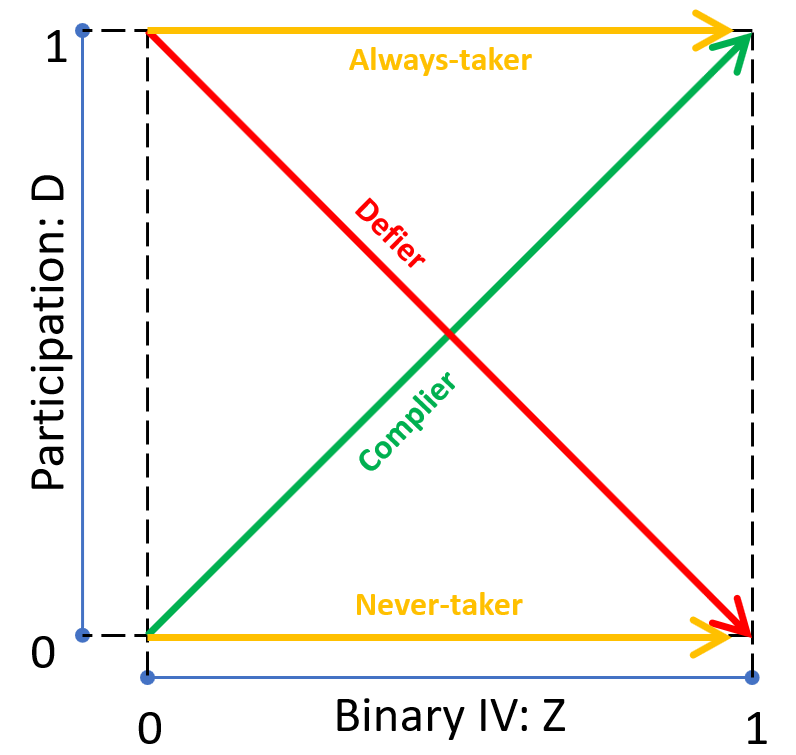
\includegraphics[scale=0.4]{images/localtreatmentclass.PNG}
\end{center}
 
Now, define $D_0 = \mathbb{I}\{\psi(0,V)>0\}$ and $D_1 = \mathbb{I}\{\psi(1,V)>0\}$. We can write the first-stage equation as: $$D = (1 - Z)D_0 + ZD_1 = D_0 + (D_1 - D_0)\cdot Z $$ and thus the second-stage equation as: $$Y = Y_0 + D_0\cdot \Delta + (D_1 - D_0)\cdot \Delta\cdot Z $$

Assuming the binary instrumental variable $Z$ is jointly independent of participation and outcome ($A2'''$), or formally, $Z\perp (Y_1,Y_0,D_1,D_0)$. Then, \begin{align*}
\E{Y\vert Z=1} & = \E{Y_0 + D_0\cdot \Delta + (D_1 - D_0)\cdot \Delta\cdot Z\vert Z=1} \\
& = \E{Y_0 + D_1\cdot \Delta \vert Z=1} \\
& = \E{Y_0 + D_1\cdot \Delta} \text{ (by } A2''')\\
& = \E{Y_0} + \E{D_1\cdot \Delta}
\end{align*}
and also,
\begin{align*}
\E{Y\vert Z=0} & = \E{Y_0 + D_0\cdot \Delta + (D_1 - D_0)\cdot \Delta\cdot Z\vert Z=0} \\
& = \E{Y_0 + D_0\cdot \Delta 
\vert Z=0} \\
& = \E{Y_0 + D_0\cdot \Delta} \text{ (by } A2''')\\
& = \E{Y_0} + \E{D_0\cdot \Delta}
\end{align*}
which implies that: $$ \E{Y\vert Z=1} - \E{Y\vert Z=0} = \E{(D_1 - D_0)\cdot \Delta} $$

This last term can be simplified with assumptions about the presence of some types of individuals in the sample. In fact, consider dividing the last term in the groups defined above: \begin{align*}
\E{(D_1 - D_0)\cdot \Delta} & = 1 \cdot \E{\Delta\vert(D_1 - D_0)=1} \cdot \Prob{(D_1 - D_0)=1} \quad \text{ (compliers)}\\
& - 1 \cdot \E{\Delta\vert(D_1 - D_0)=-1} \cdot \Prob{(D_1 - D_0)=-1} \quad \text{ (defiers)}\\
& + 0 \cdot \E{\Delta\vert(D_1 - D_0)=0} \cdot \Prob{(D_1 - D_0)=0} \quad \text{ (others)}
\end{align*}
and assume that there are no defiers in the sample, formally, that $\Prob{D_1 - D_0=-1}$ is equal to 0. Then, we get: $$\E{(D_1 - D_0)\cdot \Delta} = \E{\Delta\vert(D_1 - D_0)=1} \cdot \Prob{(D_1 - D_0)=1} $$
$$\Leftrightarrow \frac{\E{(D_1 - D_0)\cdot \Delta}}{\Prob{(D_1 - D_0)=1}} = \E{\Delta\vert(D_1 - D_0)=1} $$ where the last term is the average treatment effect conditional on being a complier. In order to compute it, we need to know the probability of being a complier. Using the $A2'''$ assumption, one can show that: $$
\Prob{(D_1 - D_0)=1} = \E{D\vert Z=1} - \E{D\vert Z=0} $$ Finally, using the implication above, we have: $$LATE\equiv \E{\Delta\vert(D_1 - D_0)=1} = \frac{\E{Y\vert Z=1} - \E{Y\vert Z=0}}{\E{D\vert Z=1} - \E{D\vert Z=0}} $$ which is called the Local Average Treatment Effect but actually only means the ATE for compliers.

This estimator has been heavily criticized due to the fact that it depends on the instruments chosen. In fact, the subpopulation of interest (compliers) can change if $Z$ is different. For example, consider the unemployment training program, where the instrument would be a coupon of 500\$ to selected individuals. Then, for a higher coupon value, say of 1000\$, the number of compliers would change for sure, making the estimator very different.

\subsubsection{Continuous IV}

Now, assume that the instrument is continuous. We have the following two-stage model:\begin{align*}
\text{(2nd stage): } Y & = Y_0 + \Delta\cdot D \\
\text{(1st stage): } D & = \mathbb{I}\{p(Z) > V\}
\end{align*} where $p(\cdot)$ is the propensity score as used in the previous sections. First, note that in this context, the no defiers condition in the binary IV case is equivalent to the threshold structure in the first-stage of this model. Second, one could assume wlog that $V\sim U[0,1]$.

As in the previous subsection, start by looking at: \begin{align*}
\E{Y\vert Z=z} & = \E{Y_0 + \Delta\cdot D \vert Z = z} \\
& = \E{Y_0} + \E{\Delta\cdot D \vert Z = z} \\ 
& = \E{Y_0} + \E{\E{\Delta\vert Z, V} \cdot D \vert Z = z} \\
& = \E{Y_0} + \E{\E{\Delta\vert V} \cdot \mathbb{I}\{p(z)>V\}} \text{ (by } A2''') \\ 
& = \E{Y_0} + \int_0^{p(z)}\E{\Delta\vert V=v} \D v 
\end{align*} 
Then, by Leibniz' rule: $$\partial_z \E{Y\vert Z=z} = \E{\Delta\vert V=p(z)}\cdot \partial_zp(z) $$ $$\Leftrightarrow \frac{\partial_z \E{Y\vert Z=z}}{\partial_zp(z)} = \E{\Delta\vert V=p(z)} $$ which is the analog result to the LATE estimator in Angrist and Imbens' work. In words, the right-hand side term is the marginal treatment effect for the population that is indifferent between participating in the program or not for a given $z$. The left-hand side term is the instrumental variable at the point $z$. Using $p$ in place of $p(z)$ we get: $$ \E{\Delta\vert V=p} = \partial_z \E{Y\vert P=p}$$ which we can use to get the global average treatment effect, as the integral over the marginal treatment effect for individuals that are indifferent at each level of $p$: $$ATE = \int_0^1 \E{\Delta\vert V=p}\D p = \int_0^1 \partial_z \E{Y\vert P=p}\D p = \E{Y\vert P=1} - \E{Y\vert P=0} $$

This strategy has also been heavily criticized, this time based on the fact that it should be impossible to observe propensity score of exactly 1 and 0. In fact, if one uses a parametric model to estimate $p(\cdot)$, then identification would only come for $Z=\pm \infty$. We call this issue identification at infinity.

\section{Distributional effects}

As we have seen, the main underlying point of interest in the previous sections was the estimation of an "average" treatment effect. If this is important, one could also be interested in studying the impact of the treatment across the whole distribution of outcomes, not only the mean. For example, answering questions such as whether a treatment increases or decreases inequality can only be done by looking at the entire distribution. There are multiple ways to study these questions, three of them will be studied here: experiments settings (everyone has to participate), quantile regressions and IV quantile regressions.

\subsection{Distributional tests}

Consider an experiment with perfect compliance, and assuming that $(Y_0, Y_1)\perp D$ (assumption $A2$); we can evaluate the distributional effects by comparing the distribution of outcomes between both groups (treatment and control). In particular, we have: $$F_{Y_1}(y) = \Prob{Y_1\leq y} = \Prob{Y_1\leq y\vert D = 1} = \Prob{Y\leq y\vert D = 1} = F_{Y}(y\vert D =1) $$ which is the cdf of outcomes considering only the treated individuals. In a similar way, we can get that $F_{Y_0}(y) = F_Y(y\vert D = 0)$, the cdf of outcomes in the control group. These two elements can be estimated using their frequentist analogs: $$\hat F_{Y_1}(y) = \frac{1}{n_1}\sum_{i=1}^{n_1} \mathbb{I}\{Y_i \leq y\} \quad \text{ and } \quad \hat F_{Y_0}(y) = \frac{1}{n_0}\sum_{i=1}^{n_0} \mathbb{I}\{Y_i \leq y\}$$
But how can we compare these two functions?

\subsubsection{Comparing distributions}

In order to compare both estimated distributions, we can look at two main ways: first, we could look at the social welfare derived from each, second, we could look at their stochastic order.

The social welfare analysis relies on computing (estimating) the value of social utility, based on the utilitarian social welfare function defined as: $$W(u, F) = \int u(y)f(y)\D y $$ where $u(\cdot)$ is the utility derived from the outcome $y$. Once this object is estimated, we want to check if $W(u, F_{Y_1})\geq W(u, F_{Y_0})$. However, the utility function is not an object that is known to the researcher, let alone individuals. We typically assume that $u'\geq 0$ (non-decreasing utility) and that $u''\leq 0$ (concave utility), but fundamentally, this problem cannot be solved.

An alternative way would be to look for mathematical properties of distribution rankings. In particular, we are interested in identifying the relation between both distribution among three types of rankings: equality (EQ), first-order stochastic dominance (FOSD) and second-order stochastic dominance (SOSD).
\begin{definition}[Distribution rankings]
Let $F_{Y_1}$ and $F_{Y_0}$ be the cdfs of the treatment and the control groups respectively.\begin{itemize}
\item\textbf{(EQ):} The distributions are equal if and only if $F_{Y_1}(y) = F_{Y_0}(y)$ for all $y$.
\begin{itemize}
\item[$\Rightarrow$] This property implies that for any utility function $u(\cdot)$, $W(u, F_{Y_1})= W(u, F_{Y_0})$
\end{itemize}
\item\textbf{(FOSD):} A distribution ($F_{Y_1}$) first-order stochastically dominates another ($F_{Y_0}$) if and only if $F_{Y_1}(y) \leq F_{Y_0}(y)$ for all $y$.
\begin{itemize}
\item[$\Rightarrow$] This property implies that for any non-decreasing utility function $u(\cdot)$, $W(u, F_{Y_1})\geq W(u, F_{Y_0})$
\end{itemize}
\item\textbf{(SOSD):} A distribution ($F_{Y_1}$) second-order stochastically dominates another ($F_{Y_0}$) if and only if $\int_{-\infty}^{y} F_{Y_1}(x)\D x \leq \int_{-\infty}^{y} F_{Y_0}(x)\D x$ for all $y$.
\begin{itemize}
\item[$\Rightarrow$] This property implies that for any non-decreasing and concave utility function $u(\cdot)$, $W(u, F_{Y_1})\geq W(u, F_{Y_0})$
\end{itemize}
\end{itemize}
\end{definition}

\begin{center}
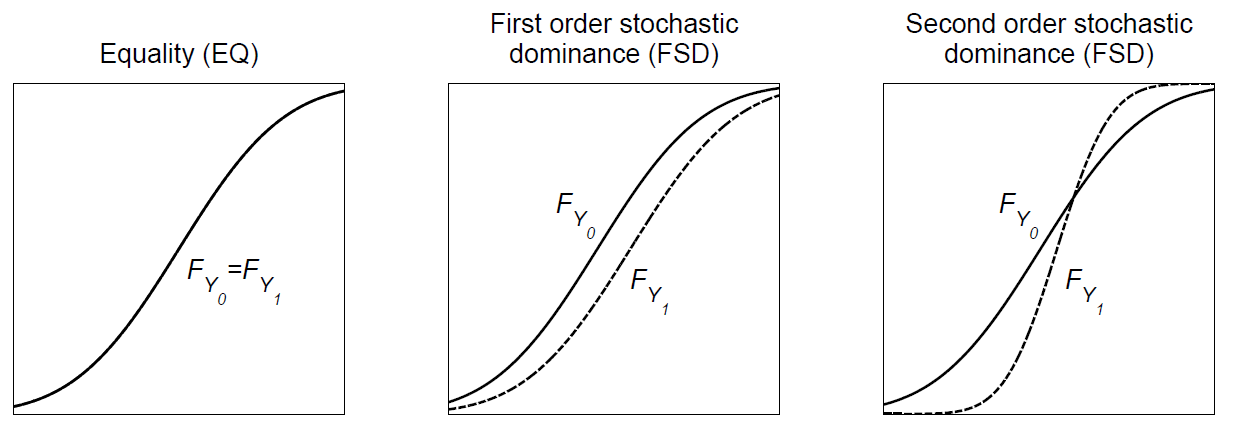
\includegraphics[scale=0.42]{images/distcompare.PNG} 
\end{center}

\subsubsection{Kolmogorov-Smirnov Test}

We've seen in the subsection just above the many ways to compare two distributions of outcome theoretically. However, because one never actually observes these distributions, we need to find a way to use the data to say something about he rankings between these. On way to empirically test whether distributions are EQ, FOSD or SOSD is using the so-called Kolmogorov-Smirnov test. This test is divided in three, each one testing for a particular relation.

\begin{definition}[Kolmogorov-Smirnov Test]
Let $Y_1$ and $Y_0$ be the outcomes of a randomized experiment ($i =1$ defines the treatment group while $i=0$ is the control group).

If the null hypothesis is $H_0: F_{Y_1} = F_{Y_0}$ (EQ hypothesis), then: $$T_{eq} = \left(\frac{N_1\cdot N_0}{N}\right)^{1/2} \cdot \sup_{y} \left\lbrace\vert \hat F_{Y_1}(y) - \hat F_{Y_0}(y)\vert\right\rbrace $$

If the null hypothesis is $H_0: F_{Y_1} \operatorname{FOSD} F_{Y_0}$ (FOSD hypothesis), then: $$T_{fosd} = \left(\frac{N_1\cdot N_0}{N}\right)^{1/2} \cdot \sup_{y} \left\lbrace\hat F_{Y_1}(y) - \hat F_{Y_0}(y)\right\rbrace $$

If the null hypothesis is $H_0: F_{Y_1} \operatorname{SOSD} F_{Y_0}$ (SOSD hypothesis), then: $$T_{sosd} = \left(\frac{N_1\cdot N_0}{N}\right)^{1/2} \cdot \sup_{y} \left\lbrace \int_{-\infty}^y (\hat F_{Y_1}(x) - \hat F_{Y_0}(x))\D x\right\rbrace $$
\end{definition}

In words, this test looks at the value of a function of $y$ for which the difference (in the measure of interest, depending of the null) in the two distributions is the greatest. If the variable $Y$ is continuous, then the distribution of $T_h$ (where $h$ is the null hypothesis) is known. However, if $Y$ is not a continuous variables (there is positive probability at $Y=0$), then one should use a bootstrap technique to test the hypothesis.

The bootstrap method is quite simple to grasp: by computing the test statistic on a resampled set of observations a high enough number of times, one can estimate the actual distribution of the test-statistic, and determine if the entire-sample test statistic is statistically different. The method follows four steps:\begin{enumerate}
\item Compute $T_h$ in the original sample.
\item Assuming the null hypothesis, resample your data and compute the new statistic $T_h^b$. For example, if the null is the EQ hypothesis, assume both groups are the same.
\item Repeat step 2 for $B$ number of times.
\item Compute the $p$-value of the test as: $$p = \frac{1}{B}\sum_{b=1}^{B}\mathbb{I}\{T_h^b>T_h\} $$
\end{enumerate}

\subsection{Quantile regression}

Recall our main objective in this section is to depart from looking only at the average treatment effect to study the effect of a program. In the previous subsection, we looked at how one could study the entire distribution of outcomes. In this subsection and the following we will be interested in studying the effect on a given quantile of the distribution. This analysis can be useful if a program is targeted towards a particular subpopulation defined as a quantile, say the 25\% of poorest unemployed individuals, etc.

In order to do that, we need to assume that for any quantile $\theta$, the $\theta$-quantile of the distribution in outcomes $Y$ is linear given $D$ (participation in the treatment) and $X$ (observable covariates) such that: $$ Q_\theta (Y\vert D, X) = \alpha_0D + X\beta_0 $$ Moreover, we will assume some version of our beloved assumption $A2$, that is, either the treatment is perfectly randomized, or it is randomized based on observables $X$. In that case, we have that $(\alpha_0, \beta_0)$ satisfy: $$(\alpha_0, \beta_0) = \arg\min_{\alpha, \beta} \E{\rho_\theta(Y - \alpha D - X\beta)} $$ where the function $\rho_\theta(x) \equiv x\cdot (\theta - \mathbb{I}\{x < 0\})$ is a function that works as a weigthing function. To see that, consider the quantile $\theta = 0.25$, then \begin{align*}
\rho_{0.25}(Y - \alpha D - X\beta) & = (Y - \alpha D - X\beta)\cdot (0.25 - \mathbb{I}\{(Y - \alpha D - X\beta) < 0\}) \\ & = \begin{cases}
- 0.75 \cdot (Y - \alpha D - X\beta) & \text{ if } Y - \alpha D - X\beta < 0 \\
 0.25 \cdot (Y - \alpha D - X\beta) & \text{ if } Y - \alpha D - X\beta \geq 0
\end{cases}
\end{align*}
meaning that all observations in the lower part of the distribution (where $Y - \alpha D - X\beta < 0$) will decrease the value of the function to minimize over (which is a good thing) while the top part of the distribution will be more costly. In that way, $(\hat\alpha_0, \hat\beta_0)$ will be chosen to favor the lower part of the distribution, and will yield the $\theta = 0.25$ quantile parameters.

The following graph shows how the weighting function works for different quantiles:\begin{center}
 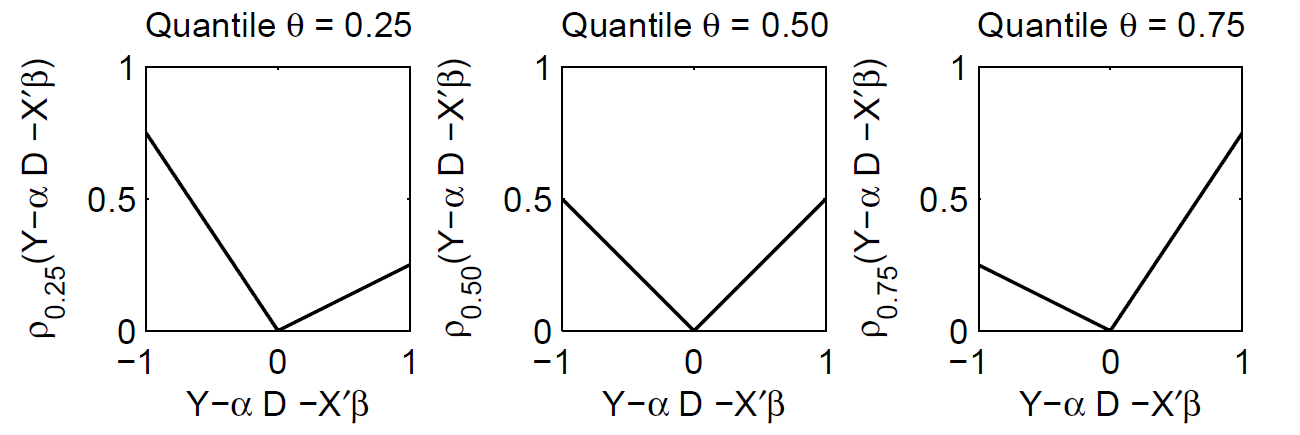
\includegraphics[scale=0.4]{images/quantilereg.PNG}
\end{center} 

Now, in order to recover the estimated parameters $(\hat\alpha_0, \hat\beta_0)$, we minimize over the sample analog of the expectation: $$ (\hat\alpha_0, \hat\beta_0) = \arg\min_{\alpha, \beta} \frac{1}{N}\sum_{i=1}^{N}\rho_\theta(Y_i - \alpha D_i - X_i\beta) $$ This estimator is called the Koenker-Bassett quantile regression estimator.

\subsection{Including Instruments}

\subsubsection{Distributional tests}



\subsubsection{Quantile regression}



\section{IV models with covariates}



\section{Differences-in-Differences (DiD)}

Often, there are reasons to believe that the treatment and control groups differ in characteristics that are unobserved, and that could be correlated with the outcomes, even after controlling for observed characteristics. In this particular case, a direct comparison between groups is not possible.

For example, consider the following question: how do inflows of immigrants affect the wages and the employment level of natives in local labor markets? To study this question Card (1990) uses the Mariel Boatlift  of 1980 (massive immigration of Cuban population to the Mariel harbor) as a natural experiment to measure the effect on uemployment of a sudden influx of immigrants. In order to measure this effect, he looked at data on unemployment for Miami and four other cities (Atl, LA, Hou and Tampa). As stressed above, those cities clearly have differences in characteristics that cannot be observed fully, and these differences will determine at least partially the dynamics of the labor force.

\subsection{Setup}

As in the previous sections, we divide individuals in two groups: the treatment group ($D=1$) and the control group ($D=0$). In addition, we differentiate between the two periods pre- and post-treatment. The pre-treatment period is indexed by $T=0$, while the post-treatment is indexed by $T=1$. Thus, our outcome variable $Y$ is now a function of the time period: $Y_{di}(t)$ is the outcome of individual $i$ at time $t$ after receiving $d$ (treatment or control).

Again, following the same intuition as in the previous sections, we are interested in measuring the effect of the treatment. In particular, consider the average treatment effect on the treated, that is the difference between the treatment and control outcomes at time $1$ for a treated individual $i$: $\E{Y_{1i}(1) - Y_{0t}(1)\vert D=1}$. However, as we know, only one outcome can be observed since one individual cannot be subject to both the treatment and the control at the same time. In fact, we can only observe the following variables:

\begin{tabular}{l|l|l|}
\cline{2-3}
 & Post-treatment ($T=1$) & Pre-treatment ($T=0$) \\ \hline
\multicolumn{1}{|l|}{Treatment ($D=1$)} & $Y_{1i}(1)$ for all $i : D_i = 1$ & $Y_{0i}(0)$ for all $i : D_i = 1$ \\ \hline
\multicolumn{1}{|l|}{Control ($D=0$)} & $Y_{0i}(1)$ for all $i : D_i = 0$ & $Y_{0i}(0)$ for all $i : D_i = 0$ \\ \hline
\end{tabular}

This means that we are missing the potential outcome $Y_{0i}(1)$ for the treated, i.e. what would have been the outcome if they did not get treated. From there, we can use three strategies.

\subsubsection{Before = after identification} 

First, we could assume that in expectations, for the treated ($D=1$), the outcome of not being treated at time $1$ is the same as the outcome of not being treated at time $0$, that is, we are assuming that without treatment, the average outcome does not change with time. More formally, this assumption states: $\E{Y_0(1)\vert D=1} = \E{Y_0(0)\vert D=1}$. Using that fact, we can recover the ATT as defined above: \begin{align*}
\E{Y_{1i}(1) - Y_{0t}(1)\vert D=1} & = \E{Y_{1i}(1)\vert D=1} - \E{Y_{0t}(1)\vert D=1} \\
& = \E{Y_{1i}(1)\vert D=1} - \E{Y_{0t}(0)\vert D=1} \quad \text{ by assumption.}
\end{align*} Obviously, one should first consider if this assumption would make sense in the setting studied.

\subsubsection{Treated = control identification}

Second, we could assume that in expectations, for the treated, the outcome of not having been treated at time 1 is the same as the outcome of not having been treated at time 1 for the control. That is, we are assuming that without the treatment being administered at time $1$, both groups would be the same. Or more formally, $\E{Y_0(1)\vert D=1} = \E{Y_0(1)\vert D=0}$. Again, using that fact, we can recover the ATT as defined above: \begin{align*}
\E{Y_{1i}(1) - Y_{0t}(1)\vert D=1} & = \E{Y_{1i}(1)\vert D=1} - \E{Y_{0t}(1)\vert D=1} \\
& = \E{Y_{1i}(1)\vert D=1} - \E{Y_{0t}(1)\vert D=0} \quad \text{ by assumption.}
\end{align*} Obviously, one should first consider if this assumption would make sense in the setting studied.

\subsubsection{DiD identification}

Finally, one could assume that in expectations, the effect of not receiving the treatment at time 1, is the same for the treated and control groups. That is, if the treated did not get the treatment, they would have seen the same evolution in their outcome. Formally, we are assuming that: $\E{Y_0(1) - Y_0(0)\vert D=1} = \E{Y_0(1) - Y_0(0)\vert D=0}$. And using this assumption, we can recover the ATT as defined above: \begin{align*}
&\E{Y_{1i}(1) - Y_{0t}(1)\vert D=1} \\  = &\E{Y_{1i}(1)\vert D=1} - \E{Y_{0t}(1)\vert D=1} \\
 = &\E{Y_{1i}(1)\vert D=1} - \E{Y_{0i}(0)\vert D=1} + \E{Y_{0i}(0)\vert D=1} - \E{Y_{0t}(1)\vert D=1} \\
 = &\E{Y_{1i}(1)\vert D=1} - \E{Y_{0i}(0)\vert D=1} - \E{Y_{0t}(1) - Y_{0i}(0)\vert D=1} \\
 = &\E{Y_{1i}(1)\vert D=1} - \E{Y_{0i}(0)\vert D=1} - \E{Y_{0t}(1) - Y_{0i}(0)\vert D=0} \quad \text{ by assumption.}\\
 = &\underbrace{\underbrace{\left\lbrace\E{Y_{1i}(1)\vert D=1} - \E{Y_{0i}(0)\vert D=1}\right\rbrace}_{\text{Difference in treated}} - \underbrace{\left\lbrace\E{Y_{0t}(1)\vert D=0} - \E{Y_{0i}(0)\vert D=0}\right\rbrace}_{\text{Difference in control}}}_{\text{Difference-in-differences}}
\end{align*}

\subsection{Estimation by sample means}

\subsubsection{Panel data}



\subsubsection{Repeated cross-sections}



\subsection{Estimation by regression}

\subsubsection{Panel data}



\subsubsection{Repeated cross-sections}



\subsection{Threats to validity}

\subsubsection{Compositional differences}

In repeated cross-sections, we could be worried about the composition of the population under study changing across cross-sections. In order to test for that, we could look at the distribution of $(D, X)$ in all samples and we would look for them to be similar.

\subsubsection{Non-parallel dynamics}

For any type of data, we could also be worried about how our main assumption for the DiD estimator could fail. In particular, if the dynamics of the outcome depends on unobservables, the assumption would fail. In order to test for that, we could run a falsification test by applying a DiD analysis on the period before the first period (period $-1$ to $0$). If our assumption holds, it should be that this DiD estimator is not statistically different from 0.

\chapter{Qualitative Dependent Variables}

\section{Motivation}

In some applications, the policy-relevant question relies on the analysis of a binomial or multinomial variable. In that case, a linear regression can mix up the results by not accounting for the given values of the dependent variable. For example, if $Y$ can only take values of 1 and 0, a linear regression estimate of $0.5$ would make no sense.

As a more general example, consider the question of female participation in the labor force. If a woman participates, then the variable of interest $Y=1$, if she does not, then $Y=0$. Assume that we believe that this participation depends on other variables such as the number of kids below the age of 6, the age, the level of education and the non-wife income of the household. Then, we want to estimate $\E{Y\vert X}$, that is the expected value of $Y$ given $X$ where $X$ contains all the variables discussed above. Since the variable $Y$ is discrete, we can decompose this expectation into probabilities: $$\E{Y\vert X} = 1\cdot \Prob{Y = 1\vert X} + 0 \cdot \Prob{Y = 0\vert X} $$ $$\Leftrightarrow \E{Y\vert X} = \Prob{Y = 1\vert X} $$ which is a probability regression on $X$.

The linear probability model (using OLS) would be to estimate the probability as a linear function of variables: $$\Prob{Y = 1\vert X} = X\beta $$ However, this model could give results not consistent with the qualitative interpretation of $Y$. In fact, this probability could be negative or above one. One solution to that problem would be to assume the specification of $Y$ depends on inputs in the following: $$Y = \mathbb{I}\{X\beta + U > 0\} $$ Therefore we have that:\begin{align*}
\E{Y\vert X} = \Prob{Y = 1\vert X} & = \Prob{X\beta + U > 0}\\
& = \Prob{U > X\beta} = 1 -  \Prob{U < X\beta}
\end{align*}
Then estimate this probability using the properties of the distribution of $U$. Given that we are now estimating a probability using probabilities, we escape the issues of finding results lower than 0 or greater than 1. In the rest of the section, we explore three possible ways to assume or estimate the distribution of $U$.

\subsection{Probit}

The probit model is the binary choice estimator assuming that $U$ is distributed as a normal with mean zero and variance $v$. Define $\Phi(z)$ as the cdf of the normal distribution $N(0, v)$, such that: $$\Phi(z) = \frac{1}{\sqrt{2\pi}}\cdot\int_{-\infty}^{z}\exp(-v^2/2)\D v $$
Therefore the probability of $Y=1$ becomes $\Prob{Y = 1\vert X} =  1 - \Phi(X\beta)$ and intuitively, the probability that $Y=0$ is $\Phi(X\beta)$.

\subsection{Logit}

In the same way, instead of using a normal distribution, one could use the logistic distribution. Both distributions are quite similar: the logistic distribution has slightly fatter tails, but it also has a closed-from solution. Denote $\Lambda(z)$ as the standard logistic distribution cdf. We have: $$\Lambda(z) = \frac{\exp(z)}{1 + \exp(z)}$$ and thus the probability model yields $\Prob{Y = 1\vert X} = 1 - \Lambda(X\beta)$ and $\Prob{Y = 0\vert X} = \Lambda(X\beta)$.

\subsection{Nonparametric regression}

Finally, instead of using assumptions on the distribution of $U$, one could use nonparametric regression which applies for binary dependent variables as well. This approach might be interesting in some settings where heterogeneity or endogeneity could play a key role in the underlying model. In fact, by assuming a parametric form on the error term $U$, one rules out the interpretation that the model is only a reduced-form version of a heterogeneous population; or that one or more variables are endogenous with $U$. This chapter will not focus on this method.

\section{Estimation}

\subsection{Maximum Likelihood}

Suppose that $(Z_1,...,Z_n)$ is a random sample drawn iid from a distribution with density $f(Z,\beta)$, where $\beta$ is not observed. Since the data is iid, we can compute the joint density of the sample as a product of individual densities. Formally, $$f(Z_1, ..., Z_n; \beta) = \prod_{i=1}^n f(Z_i,\beta)$$ This object is referred to as the likelihood of the sample, implying that it is the ex-ante probability of observing this exact draw of the joint distribution.

However, as stated above, since $\beta$ is unknown, the likelihood of the sample cannot be computed. For a given $\beta = b$, we could still compute a value of the likelihood. Therefore, we could find the value of $b$ that maximizes the likelihood of the sample, or in other words, the value of $b$ that would make this exact sample draw the most likely ex-ante. This is the maximum likelihood estimator, $\hat\beta_{ML}$, defined as: $$\hat\beta_{ML} = \arg\max_{b} L(b)\equiv \prod_{i=1}^n f(Z_i,b) $$ Since the likelihood cannot be negative, this problem is equivalent to maximizing over the log of the likelihood, conveniently called log-likelihood $\mathcal{L}(b) = \ln(L(b))$. Therefore, we have:$$ \hat\beta_{ML} = \arg\max_{b} \mathcal{L}(b) \equiv \sum_{i=1}^n \ln\left(f(Z_i, b)\right) $$

It can be then proven that the maximum likelihood estimator is $\sqrt{n}$-CAN, meaning it converges in distribution to a normal distribution at a $\sqrt{n}$ rate.

\subsection{Interpretation}

Consider a simple probit model such that $P\equiv \Prob{Y =1\vert X} = \Phi(\beta_0 + \beta_1X)$. 

If $X$ is a continuous variable, then we have that: $$\frac{\partial P}{\partial X} = \beta_1\cdot \phi(\beta_0 + \beta_1X) $$ where $\phi$ is the pdf of $\Phi$, the normal distribution cdf. Since a density is always positive, the derivative will always have the same sign as $\beta_1$, however, they do not have the same value. As a generalization, we have that the coefficient is equal to $\phi(x'\beta)\beta_j$.

If $X$ is a discrete variable, the situation is slightly different as we cannot take the derivative of the probability with respect to $X$. Nonetheless, we are also not interested in infinitesimal changes in $X$, but rather discrete jumps. Therefore, we want to know: $$\Delta P(X) \equiv \Phi(\beta_0 + \beta_1) -  \Phi(\beta_0)$$ for a change of $X$ from 0 to 1. Again, the sign will be the same as $\beta$ since a cdf is monotone and increasing, but the value will be different. As a generalization, we have that the coefficient is equal to $\Phi(x'\beta + \beta_j) - \Phi(x'\beta)$.

The interpretation of both formulas is the same as in the models we know, however in these cases, the value of these coefficients depends on the value of non-varying inputs ($x'$ in the general formulas above). In practice, these are estimated given the average value of all other inputs.

\subsection{Testing}

\subsubsection{Individual parameter testing}

The $z$-statistic and its associated $p$-value displayed in any program like Stata have the exact same interpretations as their analogs in the OLS case. A coefficient is significant if it $p$-value is lower than 0.05, and its $z$-stat is higher than 1.96 in absolute value.

\subsubsection{Multiple parameter testing}

In order to test for the significance of multiple parameters, we use the likelihood ratio test. The null hypothesis $H_0$ is that $r$ coefficients are equal to 0. We want to test it against $H_1$, that at least one is non-zero. In order to test this, we define a ``restricted'' model, where the $r$ coefficients are set to 0 (hence the restriction), while the unrestricted model includes these parameters freely. We denote the two sets of parameters as $\hat\beta_R$ and $\hat\beta_U$ respectively. Finally, we denote as $L(\cdot)$ the likelihood function, yielding the value of the likelihood of the model, for a given set of parameters.

Then, the likelihood ratio test is based on comparing both likelihoods using the statistic $R = \left(\frac{L(\hat\beta_U)}{L(\hat\beta_R)}\right)^2$, or equivalently, its log: $$ LR \equiv 2 \cdot \left( \ln L(\hat\beta_U) - \ln L(\hat\beta_R) \right) \sim \chi_r^2 $$ We reject the null if $LR > q_{.95}(\chi_r^2)$, implying that the likelihood of the unrestricted model is so high compared to the other that it must be different.

\section{Ordered Dependent Variable}

\subsection{Ordered Probit}

Sometimes, the dependent variable is not only categorical but also ordered, meaning that it follows a progression in intensity. Examples include the number of cars in a household, the highest educational degree attained, votes, indices of democracy, etc.

In that case, we will need to partition the estimated function such that each region corresponds to particular value of $Y$. For example, consider the number of cars in a household could be 0, 1 or 2. We need to estimate both a function and cutoffs so that: $$Y = \begin{cases}
0 & \text{ if } Y^* \leq c_1 \\
1 & \text{ if } c_1 < Y^* \leq c_2 \\
2 & \text{ if } c_2 < Y^*
\end{cases} $$ where $Y$ is the observed decision of the household.

Suppose that $Y^* = X\beta + \varepsilon$, where $\varepsilon\sim N(0,1)$. Then, we could compute the following probabilities:\begin{itemize}
\item $\Prob{Y = 0\vert X} = \Prob{Y^* \leq c_1\vert X} = \Prob{X\beta + \varepsilon \leq c_1\vert X} = \Prob{ \varepsilon \leq c_1 - X\beta \vert X} $
\item[] $ = \Phi(c_1 - X\beta)$
\item $\Prob{Y = 1\vert X} = \Prob{c_1 < Y^* \leq c_2\vert X} = \Prob{ c_1 - X\beta < \varepsilon \leq c_2 - X\beta \vert X} $
\item[] $ = \Phi(c_2 - X\beta) - \Phi(c_1 - X\beta)$
\item $\Prob{Y = 2\vert X} = \Prob{c_2 < Y^* \vert X} = \Prob{c_2 < X\beta + \varepsilon \vert X} = \Prob{ \varepsilon > c_2 - X\beta \vert X} $
\item[] $ = 1 - \Phi(c_2 - X\beta)$
\end{itemize}

\subsection{Censored Regression (Tobit)}



\section{Nonparametric Estimation of RC models}

\subsection{Motivation}

Consider the following random coefficients model where $X$ is a scalar: $$Y = A + XB $$ such that $(A, B)\perp X$. In this model, recall that $A$ and $B$ are random variables (not fixed parameters as we usually see in econometrics). In that sense, their value will be different for any individual observation. That is why we are not interested in point estimates of their value, but rather in their joint distribution $f_{AB}(\cdot)$.

\subsection{Identification}

The main question of this subsection is therefore, how can we identify the joint density of $A$ and $B$, given the known (observed) conditional density of $Y$ given $X$?

\subsubsection{Characteristic functions}

Before going further, let's remind ourselves the definition and properties of characteristic functions. The characteristic function is an alternative way (from pdfs and cdfs) to describe a random variable $X$. In the same way that $F_X(\cdot) = \E{\mathbb{I}\{X\leq x\}}$ completely determines the behavior and properties of $X$, the characteristic function, denoted as $\phi_X(t)$, defined as: $$\phi_X(t)\equiv \E{\exp(itX)}$$ where $i=\sqrt{-1}$ is also fully informative of the behavior of $X$. In fact, the two approaches are equivalent in the sense that the characteristic function is a Fourier transform of the pdf of $X$, and vice-versa (Fourier transforms are bijective transformations).

We can also define the characteristic function of joint densities. Consider the random vector $X = [X_1\quad X_2]'$ with joint density $f_{X}(\cdot)$. Then the joint characteristic function $\phi_{X}(t)$, where $t$ is a vector of the same dimension as $X$, say $t = [t_1\quad t_2]'$, is defined as: $$\phi_{X}(t) = \E{\exp(i\cdot t'X)} = \E{\exp(i\cdot (t_1X_1 + t_2X_2)} = \mathcal{F}\left(f_{X}(\cdot; x)\right)(t)$$

Now, consider the characteristic function of the conditional distribution of $Y$ given $X$, denoted as usual $f_{Y\vert X}(\cdot ; x)$, also called the conditional characteristic function (ccf). As explained above, we define the ccf as: $$\phi_{Y\vert X}(t ; x) = \E{\exp(itY)\vert X=x} =  \mathcal{F}\left(f_{Y\vert X}(\cdot; x)\right)(t) $$

\subsubsection{Identifying $f_{AB}(\cdot)$}

Knowing the distribution of $Y$ given $X$, we want to recover the joint distribution of $(A,B)$. Starting from the ccf of $Y\vert X$, one can show that $f_{AB}(\cdot)$ is identified:
\begin{align*}
\phi_{Y\vert X}(t ; x) = \E{\exp(it(A + XB))\vert X=x} & = \E{\exp(it(A + xB))\vert X=x} \\
& = \E{\exp(it(A + xB))} \\
& = \E{\exp(itA + itxB)} \\
& = \E{\exp(itA + isB)} \quad \text{ setting }s=tx \\
& = \E{\exp(i(tA + sB)} = \phi_{AB}(t, s)
\end{align*}
which is the exact definition of the characteristic function of the random vector $[A\quad B]$.

This means that we are one inverse Fourier transform away from the joint density of $A$ and $B$. More formally: $$f_{AB}(a,b) = \mathcal{F}^{-1}\left(\mathcal{F}(f_{Y\vert X}(\cdot; X)(\cdot)\right)(a, b) $$
$$\Leftrightarrow f_{AB}(a,b) = \mathcal{T}\left(\mathcal{F}(f_{Y\vert X}(\cdot; X)(\cdot)\right)(a, b) $$

\subsection{Estimation}



\subsection{Application}



\chapter{Panel Data}

\section{Multivariate Linear Model}

\subsection{Setup}

Recall a simple multivariate linear model (the one we use all the time) such that: $Y = \alpha + X\beta + U$ where $U$ is an unobservable term. Under the Gauss-Markov assumptions, we have seen that the OLS estimator is BLUE, and the model is easily identified. In that model, we assumed that each observation in the data corresponded to a different ``individual". Now suppose that we observe a population repeatedly over time and that the same linear model applies but to each period, separately. We end up with a system of equations, the panel, indexed by $t$, such that: $$\begin{cases} 
Y_1 = \alpha + X_1\beta + U_1 \\
\quad \quad \vdots \\
Y_T = \alpha + X_T\beta + U_T
\end{cases} $$ where we observe the joint distribution of $(X_1, ..., X_T, Y_1, ..., Y_T)$, for each individual. Note that this system describes the general population model; in reality, there are $N$ such systems of equations for $N$ individuals, yielding $N\times T$ single equations. Usually, $T$ is way smaller than $N$, so we can keep using asymptotics of $N\to\infty$, however, if $T$ is comparable to $N$, we could choose either way of performing asymptotics. Note also that the usual unobservable $U$ is now indexed by $t$, meaning it is a time-process, or innovation term that follows a stochastic process.

In this new setup, there are two ways to look at the parameters of interest $(\alpha, \beta)$:\begin{itemize}
\item Time variation: if a parameter is the same in all periods for a given individual, we say that it is time-invariant. 
\item Individual variation: if a parameter changes across individuals, we say that it is individual-specific.
\end{itemize}

In the following sections, we will focus on models where there exists one parameter that is both time-invariant and individual-specific. To set this up, assume a panel model where the intercept is the parameter in question: $$Y_t = \tilde A + X_t\beta + U_t, \quad \text{ for all } t = 1, ..., T $$
Now, we separate this individual-specific term into a population average and an individual deviation. To do that, define $\alpha = \E{\tilde A}$ as the average individual effect across the population; and $A_i = \tilde A_i - \alpha$ as the individual specific deviation from the mean. We can rewrite the general panel model as: $$Y_t = \alpha + A + X_t\beta + U_t, \quad \text{ for all } t = 1, ..., T $$ We now have both time-and-population fixed parameters in $(\alpha,\beta)$ and a time-invariant, individual specific parameter in $A$. Recall that both $\alpha$ and $A$ are unknown to the econometrician. If one is interested in estimating those parameters, assumptions about their interpretation will be necessary, which the two following sections will present.

\subsection{Random Effects approach}

The Random Effects (RE) approach is the traditional way of dealing with the parameter $A$ in panel data. It relies on the interpretation that $A$, as the individual deviation from the mean intercept $\alpha$, is purely random, in the sense that it is not correlated with observable features of the individuals contained in $X$. That's where the ``random effects" name comes from: conditional on $X$, the term $A$ is a random effect on $Y$. Following this intuition, one could set both random unobservables $A$ and $U$ into one ``total error" denoted $V$. Then, if you recall the first-year econometrics class, we could apply the Feasible GLS method of estimation. 

\subsubsection{Recap of GLS}



\subsubsection{FGLS in the RE model}

The RE model works in the same way, provided we can specify the variance matrix of the total unobservable term ($V_t \equiv  A + U_t$). For that, we need a few assumptions. Let the unindexed variables denote the vector of $t$-indexed variables and $\iota_T$ be a $T$-dimensional vector of ones. The system of equations for one individual can then be rewritten as: $$Y = X\beta + V \text{ where }$$ where $V = A\iota_T + U$ and $X_t$ is a matrix of width $k+1$ (meaning there are $k$ regressors and a constant $\alpha$). We make a few further assumptions:\begin{itemize}
\item Strict exogeneity of $U_t$, or formally $\E{U_t\vert X, A} = 0$. This means that not only $U_t$ is independent of $X_t$ and $A$, but also of any past (or future) realizations of $X$. This assumption is analog to $U$ being purely random in the simple OLS case.
\item Strict exogeneity of $A$, also written as $\E{A\vert X} = 0$. This assumption is the one leading us to the RE model in the first place.
\begin{itemize}
\item[$\Rightarrow$] These assumptions yield that $\V{V\vert X} = \V{V}$ and $\cov{A, U_t} = 0$ for all $t =1, ..., T$.
\end{itemize}
\item ``Well-behaved" variance of $U_t$, meaning it is not autocorrelated ($\cov{U_t, U_s} = 0$ for any $t\neq s$) and is homoskedastic ($\V{U_t} = \sigma_U^2$ for all $t$).
\end{itemize}
These assumptions are crucial to identify the sample counterpart to the $\Omega$ matrix in the GLS estimation. In fact, we can write $\V{V}$ as $\V{A\iota_T + U\vert X}$ and denote $\V{A} = \sigma_A^2$, we get: 

$$\begin{bmatrix}
\V{A + U_1} & \cov{A + U_1, A+ U_2} & \dots & \cov{A + U_1, A+ U_T} \\
\cov{A + U_1, A+ U_2} & \V{A + U_2} & \dots & \cov{A + U_2, A+ U_T} \\
\vdots & \vdots & \ddots & \vdots \\
\cov{A + U_1, A+ U_T} & \cov{A + U_2, A+ U_T} & \dots & \V{A + U_T} 
\end{bmatrix}
$$
$$= \begin{bmatrix}
\sigma_A^2 + \sigma_U^2 & \sigma_A^2 & \dots & \sigma_A^2 \\
\sigma_A^2 & \sigma_A^2 + \sigma_U^2 & \dots & \sigma_A^2 \\
\vdots & \vdots & \ddots & \vdots \\
\sigma_A^2 & \sigma_A^2 & \dots & \sigma_A^2 + \sigma_U^2
\end{bmatrix}
$$

As stipulated in the review of the GLS estimation, we now need a way to recover an estimator for this variance matrix, which we could then plug in the FGLS estimation procedure.

To do that, perform a simple OLS on the model, to recover $\hat V$, the estimated residuals. In the equation for the variance matrix, we have seen that all off-diagonal terms were equal to $\sigma_A^2$. Therefore, we could use that fact to recover a sample average of those terms, which will be our estimator $\hat\sigma_A^2$. Formally, we have: $$ \hat\sigma_A^2 = \frac{1}{T(T-1)/2}\sum_{s>t}\sum_{t}\frac{1}{n}\sum_{i=1}^{n} \hat V_{it}\hat V_{is} $$ which is the average over all off-diagonal terms (there are $T(T-1)/2$) of the average value of these terms across the $n$ individuals. Now that we have $\hat\sigma_A^2$, we can use it to recover $\hat\sigma_U^2$, using the fact that the diagonal of $\hat\Omega$ is composed only of $\hat\sigma_A^2 + \hat\sigma_U^2$. Then,$$ \hat\sigma_U^2 = \frac{1}{T}\sum_{t}\frac{1}{n}\sum_{i=1}^{n} \left(\hat V_{it}^2 - \hat\sigma_A^2\right) $$ which is the average over all $T$ diagonal terms of the average value of these terms across $n$ individuals.

Finally, we can compute $\hat\Omega$ as $\hat\sigma_A^2 \iota_T\iota_T' + \hat\sigma_U^2I_T$, and plug it in the feasible GLS method. Then, the RE estimator will be: $$\hat\beta_{RE} = \left[\sum_{i=1}^n X_i'\hat\Omega^{-1}X_i\right]^{-1}\left[\sum_{i=1}^n X_i'\hat\Omega^{-1}Y_i\right] $$

In the end, the RE model will give you, in exchange for strong assumptions, a way to estimate $\alpha$, a time-invariant effect on $Y$. This can be very interesting when studying settings such as the effect of gender or race on outcomes. As we will see in the next period, the fixed effects estimator will not allow for estimating such effects.
 
\subsection{Fixed Effects approach}

The precedent approach relies heavily on the assumption that the individual effect $A$ is perfectly random (not correlated with $X$), however, this view of the constant individual effect is less popular now. Another way to estimate the model would be to use the time-invariance property of the unobservables to cancel them out in the model. For that, we can use two methods: first-differencing and the fixed effects transformation. Note that in these models, the effects are not less random than before, we are still talking about the exact same effects, it is just that the naming convention is bad in that sense, so remember, fixed effects ARE random variables.

\subsubsection{First-differences}

Recall that if we have only two time periods, $t=1,2$, the model is: $$
\begin{cases} 
Y_1 = \alpha + X_1\beta + A + U_1 \\
Y_2 = \alpha + X_2\beta + A+ U_2
\end{cases} $$ and using the first difference (in $t$) of the equations, we get: $$Y_2 - Y_1 =  (X_2 - X_1)\beta + U_2 - U_1 $$ $$\Leftrightarrow \Delta Y = \Delta X \beta + \Delta U $$ which has eliminated completely the time-invariant effects $\alpha$ and $A$. Moreover, this new form is similar to an OLS model, and if the Gauss-Markov assumptions are satisfied by $\Delta Y$ and $\Delta X$, the estimator $\hat\beta$ is identified and consistent. This first-differencing strategy is useful in any context of correlation between $X$ and $A$. Nevertheless, as we can see with $\alpha$, if any regressor included is also time-invariant, this strategy will equally cancel it out.

\subsubsection{Fixed-effects transformation}

Another way of removing the individual-specific and time-invariant effect $A$ is to consider only deviations from the average. In fact, define the average of a variable over time as: $\bar Y = \frac{1}{T}\sum_{t=1}^T Y_t $. Then, $\bar A = A \Leftrightarrow A - \bar A = 0$. By applying this transformation in our complete model we also remove $\alpha$ and $A$ completely:$$
\begin{cases} 
Y_1 - \bar Y = \alpha - \bar\alpha + (X_1 - \bar X)\beta + A - \bar A + U_1 - \bar U \\
Y_2 - \bar Y  = \alpha - \bar\alpha + (X_2 - \bar X)\beta + A- \bar A + U_2- \bar U
\end{cases} $$ To simplify notation, we denote the variables transformed by this fixed effects methods as $\ddot X$. In vector notation, the model can then be written down as: $$\ddot Y = \ddot X\beta + \ddot U $$
If this model satisfies the classic Gauss-Markov assumptions, estimators will be identified and consistent. However, the convergent distribution is not exactly the same as in OLS. In fact, we have that $\Sigma = \sigma_U^2(\ddot X'\ddot X)^{-1}$ which is greater than the OLS equivalent $\sigma_U^2( X' X)^{-1}$.

As in the RE model, we are interested in estimating the residual variance. Using the same reasoning, we average over the now $T-1$ observations and $n$ individuals to get: $$\hat\sigma_U^2 = \frac{1}{n(T-1)}\sum_s \sum_i \hat{\ddot{U}}_{is}^2 $$

\subsubsection{1D vs. FE}

As we've seen, both first-differencing and fixed-effects transformation deal perfectly with the presence of time-invariant individual-specific unobservables. Nonetheless, it is true that in practice, the fixed-effects approach is used more than first-differencing. This preference is due to the fact that when variables might include measurement errors, the fixed-effects transformation will reduce the bias due to that issue. Thus, whenever variables are known to potentially include errors-in-measurements, the fixed-effects transformation will yield better estimators.

\subsection{Which approach to choose?}

The two models designed around the existence of an invariant effect turned out to be similar to simple methods like OLS or GLS. Nevertheless, whether we choose one or the other relied on a single assumption: are individual unobservable, time-invariant deviations $A$ correlated with observables $X$? To sum up, it was established that if no correlation is assumed, the RE estimator will be a consistent and efficient estimator; and if a correlation was present, the FE estimator was a consistent and efficient estimator. Moreover, we can clearly see that if we were to use FE in place of RE, we would still get consistency, without efficiency. On the other hand, doing the opposite and using RE instead of FE would not yield a consistent estimator.

Using this intuition, we can derive a sort of Hausman test to elicit which model can be used. For that, define the Hausman test statistic as: $$\hat\Gamma \equiv \left(\hat\beta_{FE} - \hat\beta_{RE}\right)\widehat{\operatorname{Var}}\left[\hat\beta_{FE} - \hat\beta_{RE}\right]^{-1}\left(\hat\beta_{FE} - \hat\beta_{RE}\right)  \quad \dconv \chi_k^2 $$

\section{Nonseparable Model}

In the case of nonseparable models such as binary choice models (probit, etc.), estimation of panel data using fixed effects is not going to work out. Indeed, the presence of the time-invariant effect $A$ within a function $g(\cdot)$ implies that it is impossible to remove it by subtracting out its average across individuals. However, in the logit case, and only in the logit case, Chamberlain's approach could yield $\sqrt{n}$-CAN estimators, by considering only people that switch choices between periods (i.e. have different $Y_1$ and $Y_T$). Although interesting as an approach, the fact that it would work only within the logit setting is not satisfactory. This section will look at how nonparametric estimation could help in generalizing the fixed effects model.

\subsection{Setup}

Consider the following model: $$\begin{cases}
Y_1 = \phi(X_1, Z_1, A, U_1) \\
Y_2 = \phi(X_2, Z_2, A, U_2)
\end{cases} $$ where, as in the fixed effects approach, $A$ is correlated with either $X_t$ or $Z_t$ and $U_t$ is i.i.d. In the same way as we did in the FE model, we try to cancel out the $A$. Since we are now within a more general setting, we call this generalized differencing. 

\subsubsection{Assumption 1}

There exists $\varepsilon > 0$ such that: $$U_t\perp (\mathbb{I}\{\lVert\Delta X\rVert <\varepsilon \}\cdot\Delta X, X_1)\vert A ; \mathbb{I}\{\lVert\Delta Z\rVert = 0 \}\cdot\Delta Z; Z_1$$ meaning that conditional on $A$ and $Z_t$, the unobservable term $U_t$ is independent of past $X$ and small increments of $X$ (in short, processes of $X$).

Assuming $F(A\vert X)$ is time-invariant, we can write: $$\partial_{\xi\vert\xi=0}\E{\Delta Y\vert \Delta X = \xi, X_1 = x} = \E{\partial_x\phi(X_1, U_1, A) \vert \Delta X = 0, X_1 = x} $$

\subsection{Binary Choice model}



\subsection{Application}



\chapter{Big Data and Machine Learning}

\section{Introduction}

\subsection{Some definitions}

The statistics of big data are somewhat different from what we have seen in the previous chapters of this class. For that reason, we will need to define (even redefine) some concepts. First of all, what is big data? Consider a simple cross-section dataset. Define $n$ as the number of observations and $p$ as the number of variables observed within each record. Most often, we have worked with what we call ``tall" data, meaning we had a lot of observations $n$ and not so much variables $p$. In the same way, ``wide" data is when $p$ is bigger than $n$. Both types of dataset are computationally demanding as they grow. Now, ``big" data is a combination of both types, with big $n$ and big $p$. As you can imagine, it is very computationally demanding, and uses different techniques than what we are used to.

In the definitions of ML, we will not use the usual regression terms. Instead, we call $X$ the input variables (or predictors) while $Y$ will be the output variable (or response). Nevertheless, we still differentiate in the same way variables that are quantitative (continuous), qualitative (categorical or discrete) and ordered; usually, discrete binary variables will be set to 0/1 or -1/1 (using dummies). When $Y$ is quantitative, the ML naming convention will define prediction of $Y$ as a regression. If $Y$ is instead qualitative or ordered, prediction will be named classification. Note that this taxonomy of methods pertains to the different types in $Y$ only; whether some or all $X$ are of one type of the other will not affect this taxonomy, even though it can call for different methods. Finally, it should be known that the usage of $Y$ in the prediction process is not mandatory. It is true that it is closer in interpretation to what we have seen earlier in econometrics, but a fringe literature exists in ML where the task is instead to describe how data is organized or clustered. This is called unsupervised learning, whereas using $Y$ (as we'll mostly do) is called supervised learning.

As was just described, one goal of statistical learning (whether machine learning or simple techniques like OLS) is to predict the outcome $Y$, given an input $X$. For that, we have to make the very general assumption that $Y$ is defined as a function $f(\cdot)$ of input variables and potentially a random error $\varepsilon$. These two objects are unknown to the econometrician. Prediction is thus all about finding a ``good enough" function $\hat f$ such that the predicted outcome $\hat Y = \hat f(X)$ is the ``closest" to the actual outcomes $Y$. Another goal of statistical learning could be to understand the relationship between $Y$ and $X$, the form of $f$ or related questions. These issues fall under the definition of inference.

\subsection{Statistical Decision Theory}

\subsubsection{Quantitative output}

Let $X\in\mathbb{R}^p$ denote a real valued random input vector and $Y\in\mathbb{R}$ a real valued random output variable. Both are linked by the joint distribution $\Prob{X,Y}$. As described earlier, prediction is about finding a function $f(X)$ for predicting $Y$, given values of $X$. For that, we need to define a loss function, denoted $L(\cdot)$, that will indicate how ``close" our function is to the reality, by penalizing errors in prediction.

One potential loss function can be the squared error function, defined as $L(Y, f(X)) = [Y - f(X)]^2$. The criterion associated with that function is to choose $f$ that minimizes the expectation of the loss function. In detail, we have: $$\operatorname{EPE}(f) = \E{\left(Y - f(X)\right)^2} = \E{\E{\left(Y - f(X)\right)^2\vert X}} $$ From that last equation, we can see that minimizing the EPE is equivalent to minimizing the conditional expectation of the loss function, given $X$. And in fact, we choose: $$f(x) = \arg\max_{c} \E{(Y - c)^2\vert X = x} $$ which has the solution $f(x) = \E{Y\vert X}$. Since expectations are not available in the data, we need to estimate it using different methods (OLS, nonparametrics, etc.).

\subsubsection{Categorical output}



\subsection{Dimensionality Curse}

We have seen how the linear estimation model (OLS) has low variance but a potentially high bias, while the nearest-neighbor was at the opposite of the spectrum, having high variance but low bias. We have also seen that this issue vanishes with bigger datasets (as $n\to\infty$), the intuition being that as the number of observations increase, a given neighborhood around a point will contain more and more points, reducing variance, allowing a lower neigborhood, thus reducing bias. It turns out that this particular intuition falls completely flat when we consider higher dimensional input variables. This is called the curse of dimensionality. It can be understood and visualized in different ways.

One intuitive way is using hypercubes. Consider a $p$-dimensional hypercube starting at a target point $x$. In one dimension, capturing 80\% of the data requires a bandwidth of 0.8, in two dimensions, the same bandwidth of 0.8 will capture only 64\% of the data, in three dimensions, only 51\%, etc.  In ten dimensions, the volume covered by a 0.8 bandwidth in each dimension amounts to merely 11\% of the data. 


\section{Linear Methods for Regression}

The linear regression model assumes that the relation between output $Y$ and inputs $X$ is either linear or approximately linear. Formally, it is equivalent to writing $f(X)$ as: $$ f(X) = \beta_0 + \sum_{j=1}^p X_j\beta_j $$ where $\beta$ is the vector of unknown parameters (which yields the unknownness to $f$) and $X_j$ could be anything from:\begin{itemize}
\item observed quantitative inputs
\item transformations of quantitative inputs
\item basis expansions, yielding a polynomial representation
\item coding of categorical variables
\item interactions between inputs
\end{itemize}

\subsection{Least-squares}

Recall that the least-squares method picks the vector $\beta = (\beta_0, ..., \beta_p)$ such that it minimizes the residual sum of squares (criterion) given by $\operatorname{RSS}(\beta) = (Y - X\beta)'(Y - X\beta)$. The first-order conditions yields: $$\frac{\partial \operatorname{RSS}}{\partial \beta} = 0 \Leftrightarrow -2X'(Y-X\beta) = 0 $$ and the second-order yields: $$\frac{\partial^2 \operatorname{RSS}}{\partial \beta\partial\beta'} = 2X'X $$
Meaning that if and only if $X$ is full-rank and $X'X$ is positive definite, we obtain a unique solution: $$\hat\beta = (X'X)^{-1}X'Y$$


\subsection{Extensions of Linear regression}

The model we have just seen relies on a linear model. However, it can be that the relationship between $Y$ and $X$ is actually not linear, so that $f(X)$ is not a linear function. In this subsection, we look at ways to move our model beyond linearity by augmenting and/or transforming the inputs $X$. Formally, we look at representations of $f(X)$ such that: $$f(X) = \sum_{m=1}^{M} \beta_m h_m(X) $$ In this equation $h_m(X)$ are called basis functions, they are transformations of the inputs $X$. The global model is called a linear basis expansion, as it expands $X$ using $h_m$ but it is still linearly entering $f(X)$.

\subsubsection{Polynomial regression}

Consider basis functions $h_m(X)$ of the form $X_j^2$ or $X_jX_k$ for $j,k = 1,...,p$. We call this class of models polynomial regressions. The simplest model of this class, assuming a single input $X$, is a $p$-degree polynomial such that: $$f(X) = \beta_0 + \sum_{j=1}^p \beta_jX^j + \varepsilon $$ It is still estimated by OLS and is quite flexible, however, higher order polynomials ($p\geq 5$) can lead to strange shapes due to boundary issues (much like in the nonparametric case).

%% GRAPH

\subsubsection{Step functions}

Consider now basis functions$h_m(X)$ which would set $X$ to 0 under some condition, and $1$ otherwise, much like a threshold-based indicator function. This class of models is called step functions. A simple example would be the following: $$ h_1 = \mathbb{I}\{X < \xi_1\};  \quad h_2 = \mathbb{I}\{\xi_1 \leq X < \xi_2\};  \quad h_3 = \mathbb{I}\{\xi_2 \leq X\}$$
Then, the global model would fit a constant in each of the set of $X$ values. It is obvious in this model that the cutpoints or thresholds $\xi$ are set by choice (vs. data-driven) which leads to the question of how to choose them.

%% GRAPH

Note that since $\sum h_m = 1$, we cannot include $\beta_0$ in the global model.

\subsubsection{Regression Splines}

One could also use both previous methods to first divide the domain of $X$ into contiguous, mutually exclusive intervals (step basis functions) and second, use linear functions or even low-degree polynomials within each interval. The result would not be a step function anymore but rather a piecewise linear or polynomial function.

In the piecewise linear case, a basis expansion would look like: $$ h_1 = \mathbb{I}\{X < \xi_1\};  \quad h_2 = \mathbb{I}\{\xi_1 \leq X < \xi_2\};  \quad h_3 = \mathbb{I}\{\xi_2 \leq X\}$$ and then, for each region $m$: $h_{m+3} = X\cdot h_m(X)$. This model yields $2$ linear parameters $\times$  $3$ regions $= 6$ total parameters. Note that the three lines that will result from this model do not say anything about continuity. Since it can be a desirable property, we would need to add constraints so that the value of $f(X)$ is the same at $\xi_{m+}$ and $\xi_{m-}$. For that, we need two constraints (one for each knot), such that: $$ \beta_1 + \beta_4\xi_1 = \beta_2 + \beta_5\xi_1 $$ $$\text{ and } \beta_2 + \beta_5\xi_2 = \beta_3 + \beta_6\xi_2 $$ which will fix two parameters and leave 4 free.

%% GRAPH

In general, piecewise polynomial functions that are constrained to be continuous, but also constrained to have continuous derivatives are called order-$M$ splines with knots $\xi_j$, $j=1,..., K$. In this case, one needs to select the order of the spline, the number of the knots as well as their location to identify the model.

\subsubsection{Natural Splines}

Although regression splines allowed for flexible and interesting modeling over the data, it still has the drawbacks of polynomial regression. In particular, recall that around the boundaries, polynomial regression can yield weird erratic functions that are not desired. In order to control for that issue, a natural spline will add constraints beyond boundary knots. The intuition is that we reduce the order of the polynomials beyond some boundaries (both left and right) to eliminate the extravagant variation at the extremes of the data. By doing that, we're estimating less parameters, and that leaves us to add more knots in the center of the data such that the increased bias in the boundaries (by having lower order polynomials) is balanced out by less bias within boundaries (by having more knots).

\subsubsection{Smoothing Splines}

Another way to control for too much variation in the regression is to punish it within the objective function. Recall that the purpose of these linear methods was to minimize the residual sum of squares. In addition to that, we could add a term in the RSS that would penalize too much variation. This term will be composed of a smoothing parameter $\lambda$, which is really a ``punishment parameter" that multiplies the integral of the second derivative (squared) of the function. This intuition works because the second-order derivative of $f(X)$ represents its curvature. This process is called regularization. The new objective function is defined as: $$ \operatorname{RSS}(f,\lambda) = \sum_{i=1}^n (y_i - f(x_i))^2 + \lambda\int(f''(x))^2\D x $$
In the extreme cases, consider $\lambda = 0$, then $f$ can be any function that interpolates the data (goes exactly through all the points), regardless of its shape. If $\lambda = \infty$, no second-order derivative will be tolerated, thus leaving only linear functions in the choice set: we are back to the OLS case. It turns out that the solution to this problem is the natural cubic spline, with knots at each value of $x_i$. Intuitively, one would worry about overparameterization in this context (since we have $n$ knots), however, the penalization of excessive variation in $f$ keeps this issue in check. Moreover, in a cubic spline, the order reduction that happens at the boundaries forces $f$ to be linear.

In vector form, we have: $$\operatorname{RSS}(f,\lambda) = (Y - B\beta)'(Y - B\beta) + \lambda\beta'\Omega_n\beta $$ where $B$ is a matrix ($n\times k$) of all basis functions, meaning $B_{ij} = b_j(x_i)$ and $\Omega_n$ is the value of the integral of second derivative products, such that $(\Omega_n)_{jk} = \int b_j''(t)b_k''(s)dt$. We can recover the optimal $\beta$ easily here: $$\hat\beta = (B'B + \lambda\Omega_n)^{-1}B'Y $$ which is called the generalized Ridge regression estimator.

\subsection{Shrinkage methods}

\subsubsection{Hoderlein's presentation of the Ridge regression}

Recall that the solution to the simple OLS model given by $Y = X\beta + \varepsilon$ has the solution $\hat\beta = (X'X)^{-1}X'Y$, under some regularity conditions. One these conditions is that the matrix $X'X$ be of full rank, or in other words, there is no collinearity in the matrix. As we have seen in Lewbel's class, issues may arise also when the $X'X$ matrix is close to being collinear, this is called the near multicollinearity issue. One solution to solve this issue is to add a constant $\lambda$ to the diagonal of $X'X$. By doing this, we shift the eigenvalues of the matrix away from 0, by $\lambda$, giving them a lower bound. With this, $X'X$ becomes positive definite, regardless of the relative size of $p$ and $n$. This estimator is called the Ridge estimator: $$\hat{\beta}_{R} = (X'X + \lambda I_p)^{-1}X'Y $$
From this formula, you can observe two things. First, since $\lambda$ enters in the ``denominator", the ridge estimator will be shrunk compared to the OLS analog for any positive value of $\lambda$. As $\lambda\to 0$, we get the actual OLS estimator. Second, this reduction in the estimator is not perfect, in the sense that it creates a bias (recall that OLS is BLUE). This bias is important because it comes with the advantage of reducing variance. In fact, it can be shown that the variance of the ridge estimator is always lower than the OLS estimator. Using the ridge estimator will therefore imply a different bias-variance tradeoff than OLS, which is better then?

The Theobald theorem stipulates that there always exists a $\lambda > 0$ such that $\operatorname{MSE}(\hat\beta_R) < \operatorname{MSE}(\hat\beta_{OLS})$. In words, you could always find a ridge estimator different than OLS such that it is better than the OLS in the MSE metric.

To sum up, the intuition of this estimator is that, by allowing some bias, we can reduce variance and get an estimator with a lower MSE.

\subsubsection{Ridge regression as a shrinkage method}

An alternative view to the ridge regression is in terms of ``shrinkage" since, as we've seen, the ridge estimator is a shrunk version of the OLS estimator. The philosophy behind this alternative view is that when the number of regressors ($p$) is high, we would like to select only a few of them to ideally improve the prediction error, but also give a more palatable interpretation of the model. In this sense, the ridge regression shrinks the coefficients by imposing a penalty on their size. In fact, we can write the ridge estimator as the estimate that solves: $$\hat\beta_R = \arg\min_\beta \lVert Y - X\beta \rVert_2^2 + \lambda\sum_{j=1}^p\beta_j^2 $$ where the first norm corresponds to the classic definition of the RSS, while the second term penalizes the values taken by each parameter in the model. Thus, we have an explicit regularization of the parameters within the function to optimize.

\subsubsection{Ridge regression optimization problem}

As stressed above, the ridge regression revolves around solving:
$$\hat\beta_R = \arg\min_\beta \lVert Y - X\beta \rVert_2^2 + \lambda\lVert \beta\rVert_2^2 $$ This problem can also be seen as a constrained optimization problem of minimizing the RSS, subject to $\beta$ being in a $p$-dimensional sphere of some radius $c$ (with $c$ having a one-to-one relation to $\lambda$).

In particular, we write: $$\hat\beta_R = \arg\min_{\lVert \beta\rVert_2^2\leq c} \lVert Y - X\beta \rVert_2^2 $$
The graphical interpretation of this problem is intuitive and interesting:
\begin{center}
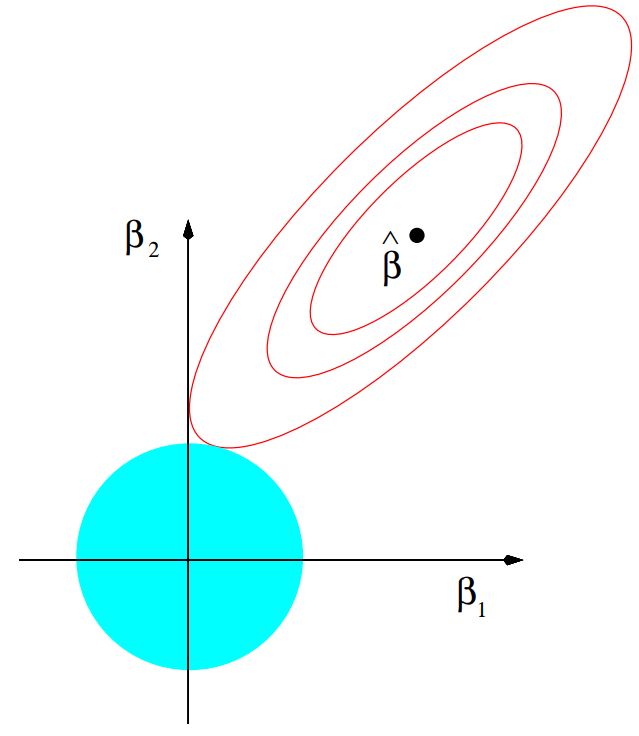
\includegraphics[scale=0.5]{images/ridgegraph.PNG} 
\end{center}
In this graph, we can see in red the level curve representation of the objective function (the RSS), while the blue circle (2D representation of the sphere) is the constraint on parameters. Then, instead of finding the point that minimizes the objective function (i.e. the eye of the objective), we look for the tangent point between the objective and the constraint sphere, which is different from $\hat\beta$, the OLS estimator.

\subsubsection{Lasso regression}

The lasso regression is another shrinkage method like ridge, with a defining difference in the norm used to constrain $\beta$. in the ridge setting, we have constrained $\beta$ to a sphere by setting its norm 2 to be lower than a given scalar $c$, formally: $\lVert \beta\rVert_2^2 \leq c$. The lasso, on the other hand, uses the norm 1 to do the exact same thing. Norm 1, denoted $\lvert \beta\rvert_1$, is the sum of absolute values of the parameters. Therefore, its formal definition is: 
$$\hat\beta_L = \arg\min_\beta \lVert Y - X\beta \rVert_2^2 + \lambda\sum_{j=1}^p\lvert\beta_j\rvert $$ or in its constrained optimization form: 
$$\hat\beta_L = \arg\min_{\lvert \beta\rvert_1\leq t} \lVert Y - X\beta \rVert_2^2 $$

In order to understand more intuitively the difference between the two estimators, we go back to its graphical representation.
\begin{center}
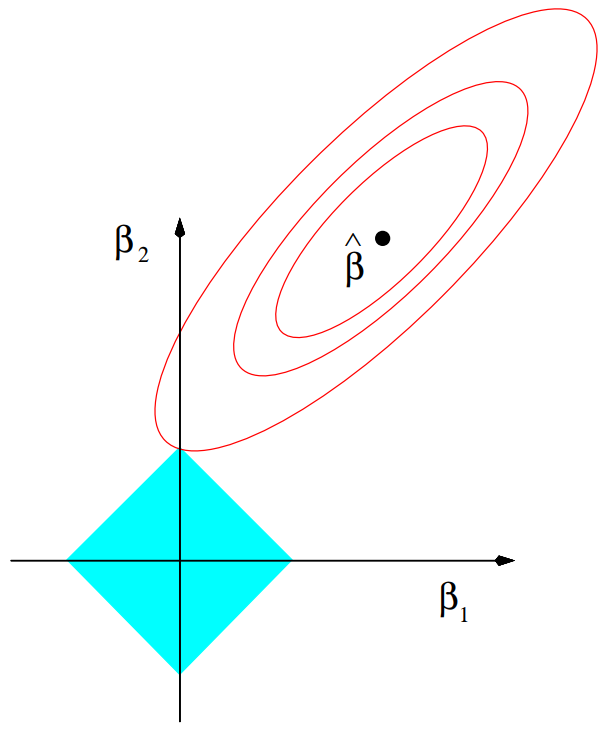
\includegraphics[scale=0.5]{images/lassograph.PNG} 
\end{center}

As you can see, the constraint area is now a diamond (whose 2D representation is a tilted square). The interpretation of the difference between this solution and the OLS has not changed. However, as is clearly shown in the graph, the lasso estimator will have a tendency to shrink some parameters all the way to 0 ($\beta_1$ is this case). In particular, if the data is organized such that $p>n$ (OLS solution is not unique and overfitting), the lasso regression will make so that only $k<n$ regressors are left, creating a sparsity in the parameter vector.

\section{Tree-based methods}

\subsection{Introduction}

Tree-based methods are a completely different approach to estimation of random variables. Its goal is to partition the feature space (input space) into a set of rectangles and fit a simple model into each of the rectangles. For example, consider a regression problem with a continuous response $Y$ and inputs $X_1$ and $X_2$, each taking values within $[0,1]$. The following graph shows how a tree could be used to estimate $Y$ using the inputs. On the left panel, you can see the process of partitioning: first, we divide the data in values of $Y$ for which $X_1 \leq t_1$ or not; then, on each side of the division, we partition again, fit a constant, etc. until our tree meets a criterion. The result of this method is shown in the right-panel.

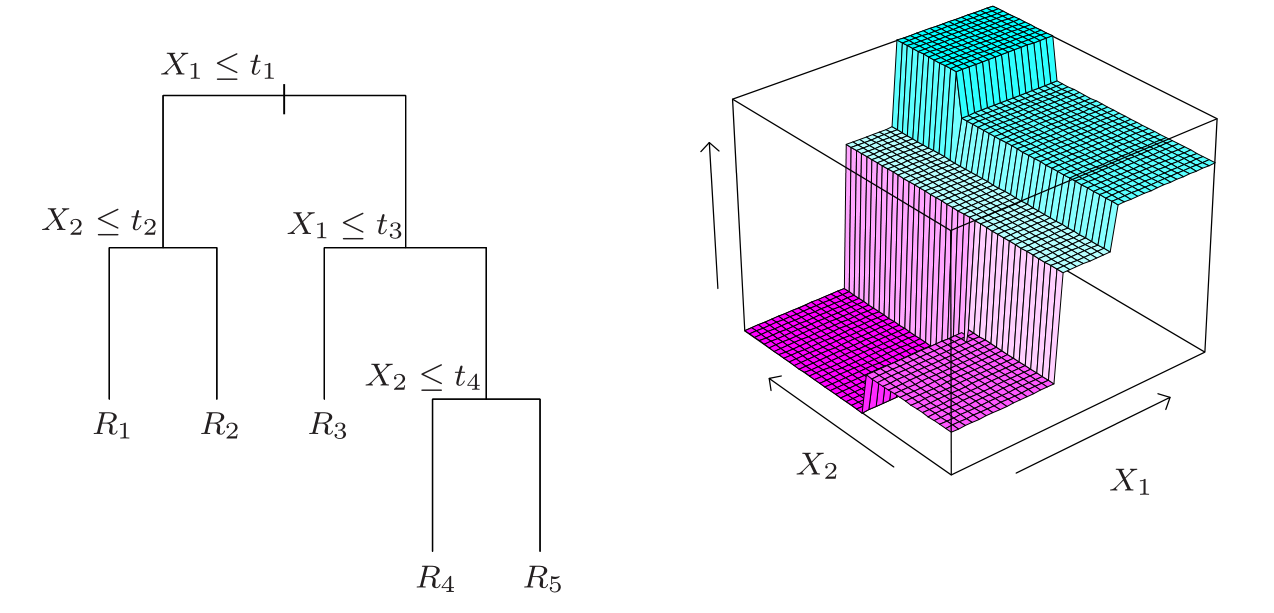
\includegraphics[scale=0.4]{images/tbmethod.png}

\subsection{Formal definition}

Let the dataset contain $N$ observations $(x_i, y_i)$ for $i = 1, ..., N$, and $x_i$ a $p$-dimensional vector $(x_i1, ..., x_ip)$. Given a partition of the $\mathbb{R}^p$ space into $M$ regions denoted $R_1, ..., R_M$, fitting a regression tree is defined as finding the function: $$f(x) = \sum_{m=1}^M c_m\cdot \mathbb{I}\{x \in R_m\} $$ such that it minimizes the RSS given by $\sum_{i=1}^N (y_i - f(x_i))^2$. This is equivalent to minimizing the RSS in each region, yielding as a result that $$\hat c_m = \frac{1}{N_m}\sum_{i\in I_m} y_i $$ or in words, the average value of $y_i$ in the region $R_m$. Note that this method is useful only when the partition is given! Finding the exact partition that would yield the lowest possible RSS is computationally infeasible. Instead, one should use a so-called ``greedy algorithm''.

\subsubsection{Greedy algorithm}

The greedy algorithm is a heuristic method of finding an optimal solution, it is called greedy because it is short-sighted and will go the nearest best solution, without realizing that there could be a better global solution by making a less optimal choice right now. In the setting of designing trees, the algorithm solves two optimization problems, one nested within the other. These are called inner and outer minimizations.

First, the algorithm starts with all the data and considers splitting a variable $j$ at a cutpoint $s$. This would create two regions $R_1(j,s) = \{X\vert X_j \leq s\}$ and $R_2(j,s) = \{X\vert X_j > s\}$. Given these regions, the algorithm solves the tree as was described in the previous section, meaning that it finds $(c_1, c_2)$ such that it minimizes the RSS. This process is the inner minimization. Then, the algorithm chooses which pair $(j, s)$ would yield the lowest RSS, among all feasible pairs. This is the outer minimization problem. All in all, this process can be formalized as finding: $$(j^*, s^*) = \arg\min_{(j,s)} \left[ \min_{c_1} RSS(y_i,c_1; R_1(j,s)) + \min_{c_2} RSS(y_i,c_2; R_2(j,s)) \right] $$ The data is now partitioned in two regions, and we repeat this process in each of them, increasing the size of the tree until a particular criterion has been met.

\subsubsection{Growing the tree}

Which criterion to choose? From what we know about statistics, growing the tree indefinitely will cause overfitting, while not allowing it to grow enough might lead to miss important features. In fact, the size of a tree will govern the complexity of the model, hence one should try to let the data guide the size of the tree.

One approach could be to evaluate the variation in the total RSS of the model after each split, and stop before a split when the RSS decrease is too low. However, this raises two issues: first, the choice of the threshold is not guided by the data, and it might not be optimal; second, this strategy is also short-sighted in the sense that a very small decrease in RSS at a given step might lead to bigger decreases in the following steps. Recall that the greedy algorithm is already short-sighted in this way, thus we might try to choose another, more robust method.

Another strategy, usually preferred, is to first grow the tree until it is large enough (say 5 nodes). Then, we would use a ``pruning'' method called cost-complexity pruning. Denote the big tree as $T_0$ and define $T\subset T_0$ as a sub-tree which could be obtained by ``pruning'' the tree $T_0$, meaning collapsing an internal node of the tree. Use $m = 1,...,M$ as an index for terminal nodes, such that the input space is partitioned in $M$ regions. Finally, let $\lvert T\rvert$ be the number of terminal nodes (regions) of $T$. Now define,\begin{itemize}
\item $N_m = \lvert\{x_i\in R_m\}\rvert$, the number of observations within a region $m$.
\item $\hat c_m = \frac{1}{N_m}\sum_{x_i\in R_m} y_i $, the constant fit in region $m$.
\item $ Q_m(T) = \frac{1}{N_m}\sum_{x_i\in R_m} (y_i - \hat c_m)^2$, the average RSS of the fit within region $m$.
\end{itemize}

The cost-complexity criterion of a tree $T$, denoted as $C_\alpha(T)$ is defined as: $$C_\alpha(T) = \underbrace{\sum_{m=1}^{\lvert T\rvert} N_m Q_m(T)}_{\text{RSS of the tree }T} + \underbrace{\alpha\cdot \lvert T\rvert}_{\text{cost of the number of regions }} $$ As you can see, this criterion contains a trade-off between the total RSS of the model (its fit) and the number of regions it creates, for a given parameter $\alpha$. A higher $\alpha$ would penalize big trees, while a lower $\alpha$ would allow for bigger trees. Therefore, $\alpha$ is key in governing this trade-off can be considered as a tuning parameter of the model. The idea behind this criterion is that for a given $\alpha$, the optimal tree is the subtree $T_\alpha\subseteq T_0$ that minimizes $C_\alpha(T)$. One can show that this tree is unique for any value of $\alpha$.

\subsection{Bagging}

The concept of bagging, or \textbf{b}ootstrap \textbf{agg}regat\textbf{ing}, is linked to the concept of bootstrapping. Recall that the main idea of bootstrapping is to assess the accuracy of parameter estimates using multiple samples from the data. The method of bagging is essentially an average over a collection of bootstrap samples. 

Formally, consider a set $Z$ containing ``training'' data $\{(x_1, y_1), ..., (x_N,y_N)\}$ where we fit a model yielding our main estimate $\hat f(x)$. In order to perform bagging, we need to first draw $B$ samples from $Z$, which we denote $Z^b$ for $b=1, ..., B$. In each sample, we fit the same model as before, this time yielding a different estimate $\hat f^b(x)$. Then, the bagging estimate is the average of all bootstrap fits: $$\hat f_{bag}(x) = \frac{1}{B}\sum_{b=1}^{B} \hat f^b(x)$$

In the tree regression setting, this estimator is interesting as each $\hat f^b(x)$ will be a different tree, displaying different features such as different partitions, but also a different size! An example on the following page:

\begin{center}
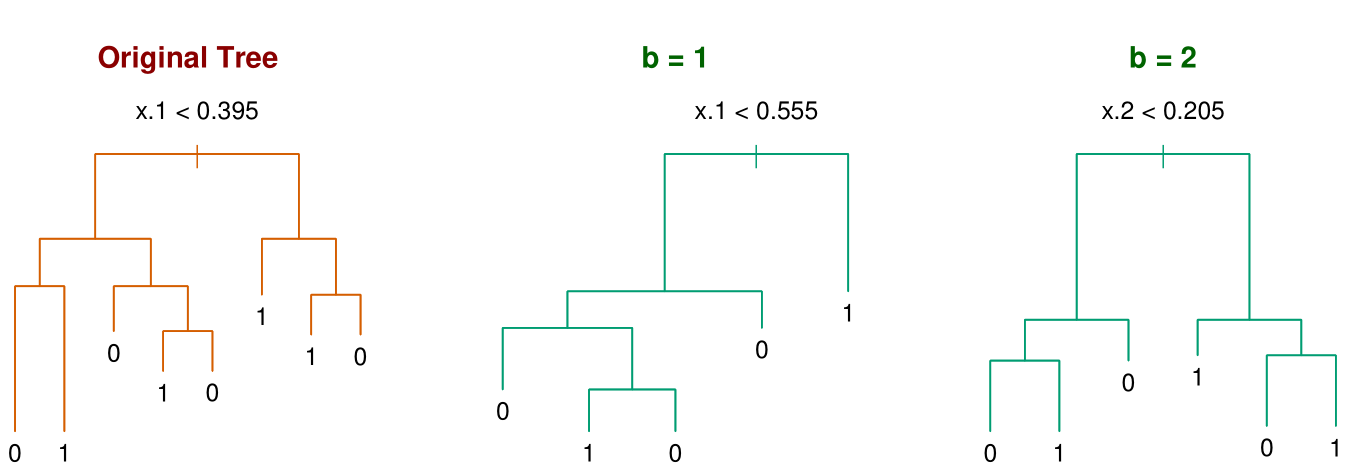
\includegraphics[scale=0.35]{images/bag1.png}
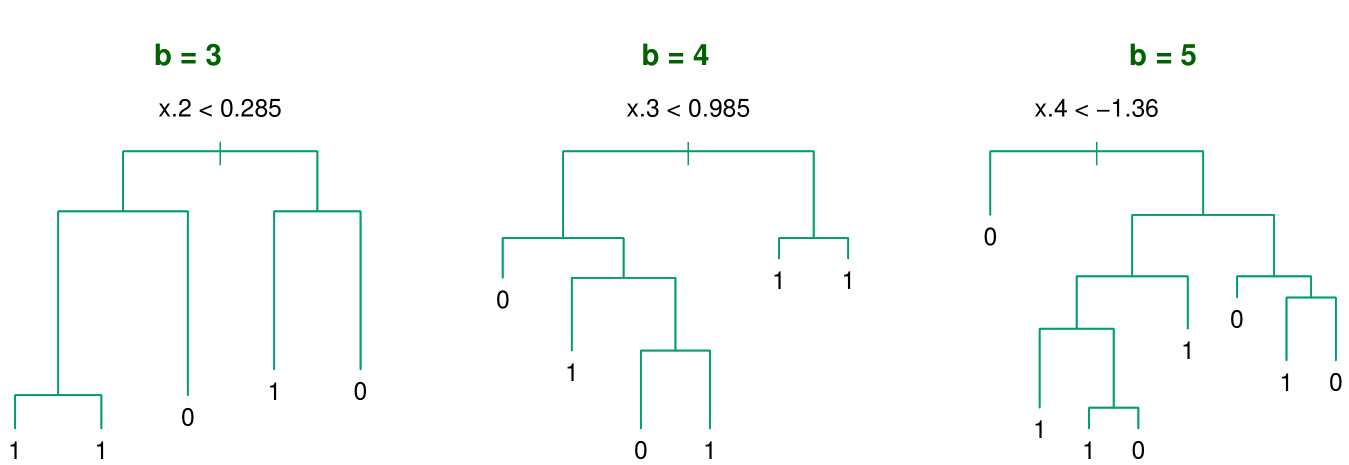
\includegraphics[scale=0.35]{images/b2.png}
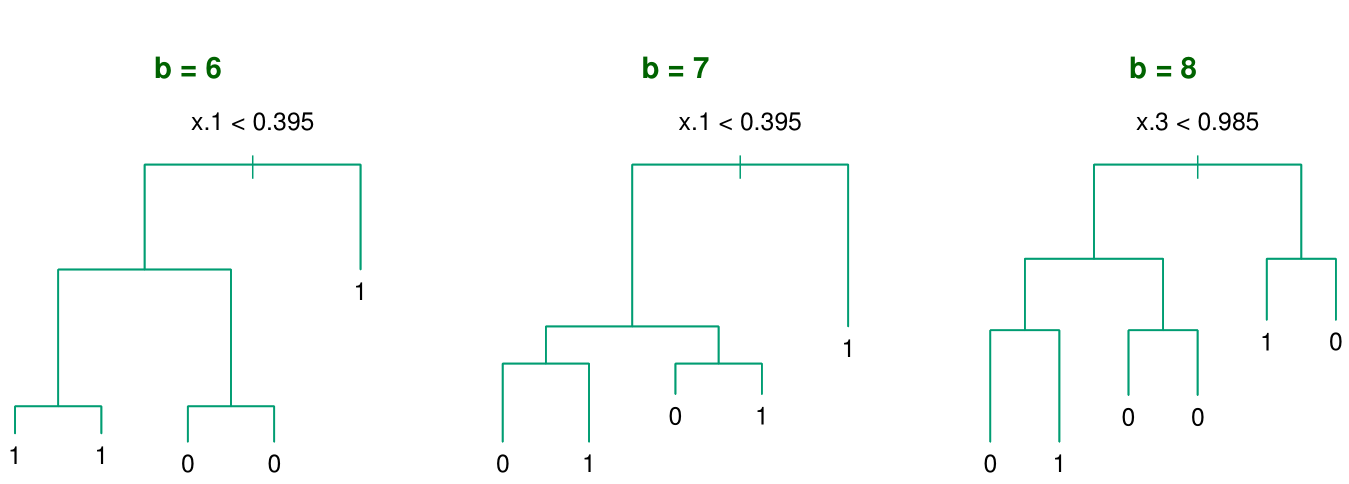
\includegraphics[scale=0.35]{images/bag3.png}
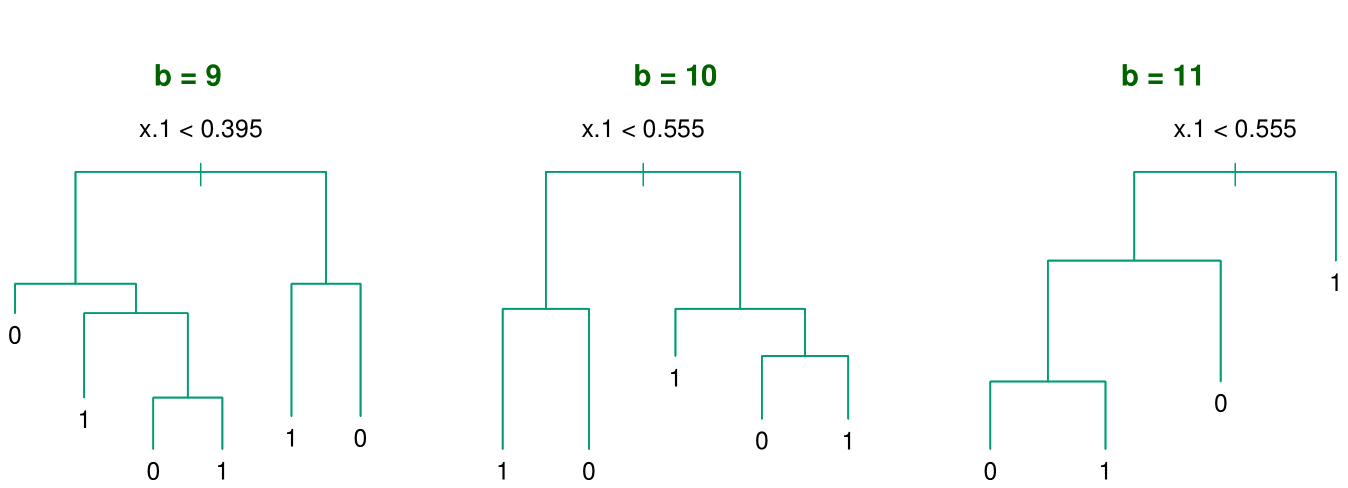
\includegraphics[scale=0.35]{images/bag4.png}
\end{center}

\subsection{Random Forests}

The random forests method is a substantial modification of bagging.  While bagging was averaging over many trees of the same type (correlated), random forests are based on averages of completely random trees so that they end up uncorrelated. To go further, consider the fact that any tree in the bagging process will have the same expected bias than any other. Thus, getting a better model from bagging means going through variance reduction, which is achieved by averaging over many trees. In that sense, random forests are not very different than bagging but allowing for uncorrelated trees will yield even lower variance than through averaging only.

Starting with a data sample of size $N$, the procedure is defined as follows: for $b = 1, ..., B$:\begin{itemize}
\item[(a).] Draw a sample $Z^b$ from the data.
\item[(b).] Grow a tree $T_b$ using $Z^b$ by repeating the following steps, until a minimum number of nodes $n_{min}$ is attained:\begin{itemize}
\item[i.] Select $m$ variables at random for the $p$ variables.
\item[ii.] Pick the best variable/split pair among the $m$ variables
\item[iii.] Split the node into daughter nodes and perform step 1.b.i again.
\end{itemize}
\item[(c).] Save output tree as $\hat f^b(x)$.
\end{itemize}
Finally, we have: $$\hat f_{rf}(x) = \frac{1}{B}\sum_{b=1}^{B} \hat f^b(x)$$

\subsection{Boosting}



\end{document}